

\section{Introduction}

In the previous chapters, we have discussed visualisation and its role in bridging the gap between data and understanding. We have applied centrality metrics to a chemical network to tell us what species are of importance and experimented in getting machine learning models to learn the chemical structure of the species in a mechanism. This final research chapter provides a (brief) overview of current mechanism reduction techniques while providing two novel alternatives to aid the process.

Science often deals with the problem of understanding complexity. Such a task may be accomplished through organisation and partitioning, for example, the learning of a new skill through chunking (breaking up a problem into manageable chunks), or the parallelisation of a sizeable mathematical problem. In cases where such methods fail, we are forced to `disregard' complexity. It is common to approximate an atom as a sphere or the value $\pi$ as 3 with little consequence to the overall result of a calculation. The process of lumping has long been used to replace a complex, changing process (e.g. Quantum Mechanics or Boundary Layer Fluid Dynamics) with a more straightforward constant process, \citep{approx}. In such cases, an approximation may be far more useful than a lengthy exact solution, or none at all provided the primary criteria/outcome is identified and optimised for (evaluated against a benchmark or standard).

Similar problems of complexity are seen within the chemistry of the atmosphere. An example is seen within the Master Chemical Mechanism (MCM v3.3.1), \citep{mcm}, this contains 1228 \ch{RO2} reactions. If written explicitly, all \ce{RO2-RO2} (gross and self) interactions would result in a total of 1,507,984 reactions. Instead, the MCM overcomes this problem by creating a \ch{ro2} pool, with which all \ch{RO2} species react. This results in a mechanism which preserves the quality of science (the primary goal of the MCM is to preserve \ch{o3} prediction) with only 0.000814 of the total possible \ch{ro2+ro2} reactions.

However, even with such simplifications, atmospheric chemical mechanisms have been increasing in size over the last ten years (\citep{defra1},\autoref{fig:webmcm}). With the ability to automate their construction, mechanisms with species numbers of the millions become possible. Although the existence of more-explicit mechanisms may improve the quality of science produced, they can cause problems for efficient computation, diagnosis and analysis. This chapter shall look at two methods in which we may simplify a mechanism by grouping species with similar reaction patterns together. These are through the use of species lifetime (\autoref{sec:lifetime}) and graph-based clustering (\autoref{sec:graphreduction}).




\section{Mechanism Reduction}

\textit{Although this chapter discusses work which can contribute to a chemists toolkit for mechanism reduction, it itself does not concern itself with this task specifically - and will not contain any work directly related to this nor analyse the results of a mechanism where the species suggested may be lumped together. Although the framework for such a task exists, this shall be left as a task for future work.  }

Currently, there exist two main reasons for trying to find species of similar chemical properties. These are searching for pysciochemical analogues within the field of cheminformatics (see \autoref{ch5}) and mechanism reduction. This chapter concerns itself with using the graph structure to group species with reactions on fast timescales, or similar connectivity patterns - a problem commonly presented in the production of a reduced (simplified) chemical mechanism. For this reason, the following section provides a short literature review on several different reduction techniques.

\subsection{Species Categories}

As with any problem, the first step to simplifying a complex task involves the partitioning data into categories. For a mechanism, we begin by observing the foci of an experiment and defining some critical (necessary) species for the task. Following these needed species (species which are required by the essential species for the chemistry to work) are identified and added. Finally, species which provide a negligible input to the aims of an experiment are labelled as redundant and often removed.  The outline of each category is given below.


\begin{itemize}
    \item \textbf{Important} - reactions or species directly related to the topic/outcome we are interested in (for the MCM this is ozone)
    \item \textbf{Needed} - reactions/species required by the important species/pathways, such that they may perform their desired function
    \item \textbf{Redundant} - those we may remove with little or no consequence to the outcome of the model. These are determined through the use of sensitivity analysis.
\end{itemize}



\subsection{Reaction Removal}
Since atmospheric chemical mechanism forms a numerically stiff system (\autoref{ch0}), a reduction in the number of reactions within a mechanism leads to a reduction in the computational burden experienced by a model each iteration forwards in time. Classically the identification of important reactions may be accomplished through the use or rate of production and loss analysis (\autoref{sec:ropa}). This allows us to filter reactions contributing less than 5\% (in the MCM reaction pathways $<5\%$ are disregarded) to the formation of any species we are interested in. Other methods using principal component analysis of the sensitivity of species (PCAS) also exist and are discussed in \citep{PCAS,wyche}.


\subsection{Species Removal}
Similar to reaction removal, the removal of species is useful because the removing or combining of species inherently reduces or simplifies the reactions within a mechanism.  This method also has added benefit of reducing the size of the jacobian matrix used to propagate the chemical system forwards. For large systems which do not use a sparse framework, storing a $n^2$ matrix in memory can prove difficult.

Many methods of species reduction are possible. The simplest of these is through the use of trial and error \citep{tur1990} (Method 1). Here the consuming reactions for a species are removed, and if the resulting deviation in results between the full and reduced mechanism is small within a certain threshold, their results are retained. The main downside to this is that it only works on a per-species level, which may be very resource-consuming for large mechanisms.

With the use of sensitivity analysis, it is possible to remove species whose reaction are much slower than the rate-determining steps of a mechanism, \citep{frenk}. However, even after removing all slow-reacting species, those on a fast timescale remain. Here the use of Quasi-Steady-State Approximation (QSSA), \citep{QSSA}, can be used to identify species associated with fast timescale reactions. QSSA works on the assumption that such species have little to no change in concentration over time - i.e. the net flux ($\dot{v_i}$) is zero. Such an assumption causes an error $\Delta c_i$ of :
\begin{equation}
    \Delta c_i = \frac{\dot{v_i}}{J_{ii}}
\end{equation}
where $J_{ii}$ is the diagonal of the Jacobian matrix. Here if the error for a species is small, the species may be removed from the mechanism.


Finally, investigation of the system Jacobian can be used to identify redundant species, which is a `capable' and `efficient' method for removing most redundant reactions and species from the MCM, \citep{QSSA}. Use of a log-normalised Jacobian to determine which species can be removed is found in the connectivity method \citep{connectivity,cm}.
Here the influence a 1\%  change in a species concentration has on the concentration of `important' species can be determined by

\begin{equation}
B_i  = \sum_j(({y_i}/{f_i})({\partial f_i}/{\partial y_i}))^2 \label{connectivity}
\end{equation}

 where $({y_i}/{f_i})({\partial f_i}/{\partial y_i})$ is element $i$ of the normalised Jacobian (see \autoref{ch3} for information about the construction of the Jacobian matrix). Through an iterative process species with a low contribution to our important species can be found and removed.


\subsection{Lumping}

Rather than removing species or reactions from a mechanism, we may combine them to form a new composite species. This is referred to as species lumping. To do this, we must first consider how we define species that are to be joined together, and then how their grouped reactions will contribute to every other species it reacts with. Some of the more general types of lumping styles are outlined below.


\subsubsection{Chemical Lumping}\label{sec:chemlump}
Mechanisms follow protocols in their generation. This produces reaction styles that many like-structured species follow in their degradation. In determining such classes, we may be able to generalise like-species reactions and group them as one.
An example of this is the Common Representative Intermediates (CRI) Mechanism (described in \autoref{sec:whycri}).  Here the `ozone production potential' of the species within the MCM is used to simplify and reduce it. This is a function of the \ch{c-C} and \ch{c-H} bond ratio of a species (its CRI index). Species with the same CRI index are lumped (grouped) into a proxy species. Alternatively, time scale analysis for species lumping has been successfully applied by  \citep{lifetime}. Here it is seen that many groups of species have rate coefficients that are identical or sufficiently similar due to the generic rules/protocols of the MCM. This results in a similar overall lifetime for species in the same group, allowing them to be lumped together with little overall consequence to the experimentation criterion.


\section{Data Setup}
Unlike manual reduction, this chapter does not concern itself with the intricacies of the chemistry behind a mechanism. Instead, we search for an automated method of simplifying the mathematical structure behind a mechanism while preserving the quality of science it represents. Although this may not directly replicate real-world scenarios, it can provide an accurate test of the robustness of a mechanism and the equations within it.
Work is carried out on the assumption that the equations within the MCM benchmark mechanisms are representative of experimental results, and in simplifying these, their usefulness in modelling the real data is preserved. This section describes the experimental setup for the experiment.


\subsection{The Mechanism}


The mechanism used is the Common Representative Intermediates (CRI) Mechanism v2.2 \citep{criv2}. This is an already reduced version of the MCM v 3.3.1, where species are grouped based on their ozone formation potential - i.e. the \ch{c-C} and \ch{c-H} ratio of bonds.
Reductions have been made on a compound-by-compound basis and compared to the MCM using a series of 5-day box-model simulations, \citep{cri}.

\paragraph*{Why further simplify the CRI network?}\label{sec:whycri}
5809 species and 17224 reactions

CRI v2.2 \citep{cri} is a mechanism of 422 species and 1261 reactions - that is 7\% of the species and 7\% of the reactions of the full MCM. Although this is significantly smaller than the full MCM, it may still prove problematic if used within a global model - for comparison the GEOS-Chem\footnote{A global 3D model of atmospheric chemistry driven by meteorology from NASA's Goddard Earth Observing System (GEOS), \citep{geos}.} standard chemistry is approximately half the size of this, \citep{geosgit}.

\subsection{The Box-Model}
The box model is an adapted version of the Dynamically Simple Model of Atmospheric Chemical Complexity (DSMACC) \citep{dsmacc,dsmaccgit}. Recent updates allow for multiple parallel runs, easy extraction of rates, fluxes and the jacobian matrix as well as a simple Ncurses (a command like semi-graphic interface) interface for loading and parsing new files.

The DSMACC model works by using the Kinetic PreProcessor (KPP), \citep{kpp}, to generate Fortran code, which can then be used to integrate the provided mechanism. As there were some issues presented a pre-pre parser code is used before running KPP. Occasionally a post parser may be required on some of the files to produce the desired output.

\subsection{Model Inputs}\label{sec:lumpinputs}
The aim of this experiment is not to replicate a specific case study or scenario. Instead, we extract all non-lumped species which appear in both CRI and the MCM and provide an assortment of initial condition concentrations to cover the entirety of the input space.

To select the initial conditions there exist several sampling styles \citep{sampling}. The most common style is the random or `Monte Carlo' approach. However, this does not guarantee a homogeneous distribution of points. A lattice or grid approach is also possible, but that can result in a large number of sample points to produce a complete distribution of the input space. To overcome this, a Latin hypercube can be used. This is a generalisation of the Latin square  -  a square matrix containing n items, arranged in such a way that they only appear once in each row and column (akin to a sudoku puzzle) \citep{lsq}. The experimental setup uses a Latin hypercube to define the initial condition range for 148 primary emitted species, and 300 simulations follow the formula below:

\begin{equation}
\text{concentration}
    \begin{cases}
      min = 100ppbv \ max=1pptv , & \mathbf{if} NO,NO_2,O_3\\
      min = 10ppbv \ max=0.1pptv , & \text{otherwise}\\
    \end{cases}
\label{eqn:icslhs}
  \end{equation}
\section{Graph Based Reduction}\label{sec:graphreduction}
It has been shown that a graph-based representation of the atmospheric chemical network proves useful in both the visual and mathematical analysis of simulation results (\autoref{chaptervis,chaptermetric}). It, therefore, follows that the network representation of mechanism may also have its uses in the simplification, and thus reduction, of chemical complexity.  This section will outline the basic methods of modularity (cluster) detection with the graph framework, the different methods in which this may be done and eventually apply it to a case example representative of the chemistry within the London environment.




\subsection{Graph Parallels}

% \textit{
% EDIT\\
% Although many graph-based methods exist within the reduction realm, most of these concentrate on the generation of skeletal methods through the building of a directed tree (a subcategory of graphs from source to target) - LIST of refs and sentence of all skeletal methods. Path flux analysis (Sun et al 2010)\\
% Instead, we may find ourselves applying graph theory to solve other reduction methods. For instance, we can trace back influence through connecting edges using Dijkstra's shortest path algorithm (CH2 ref) - analogous to the connectivity method, or a leave one out approach combined with PageRank to access the effects of removing a node.
% }

Graph structure can be used to analyse changes of reactions or relationships between species - providing an alternative representation and method to access such data. Additionally, clustering techniques may be used to locate groups of highly connected, fast reacting/strongly related species. This has applications in both understanding the data, but more importantly, chemical lumping. In creating a graph from a model simulation, we encode not only information about the chemical structure, but also the influence between species in the mechanism. By grouping species which have a strong dependence upon each other, we can simplify the provided network or mechanism.

 \subsection{Types Of Graph Clustering}
Unlike vector clustering algorithms (such as DBSCAN, UMAP and K-means - see \autoref{veccluster}), graph clustering metrics do not rely on the spatial orientation of the data to determine groups or `clusters'. Instead, these may partition the network into segments, group nodes by structural equivalence or explore the `flow' dynamics of the network.

Algorithms such as Label Propagation \citep{labelprop} and spin-glass \citep{spinglass} work by randomly assigning nodes with a property or label. This property is then transferred to its neighbours. Other algorithms such as the nested block model can decompose a graph into clusters of similar properties, \citep{communitygraph}. These are often grouped in the form of topological equivalence which can be either:
\begin{itemize}
    \item[-]\textit{structual equivalence} - vertices are similar if they have like neighbours, \citep{strueq}.
    \item[-]\textit{regular eqivalence} - retrieves nodes with similar connection patterns (e.g. parent - child node hierarchicl structures), \citep{regequiv}.
\end{itemize}
This works in a similar way to an AutoEncoder (discussed in \autoref{sec:ae}), where topological similarities are used to simplify (or encode) the network structure, in a way which it may be decoded again.

Finally, there exist a set of `flow' based models which use the network dynamics to determine the modularity of a network. These are discussed below.

\subsection{Walk/Flow-Based Clustering}
Temporal networks result in a change in the relationships between items (magnitude/type). Such changes in the network dynamics are encoded within the edges of a graph. The primary function of a random walk or `flow' algorithms is to capture the changes between the real-world systems represented by the network.

In \autoref{sec:silo}, the silhouette coefficient was used to compares the vector position of clusters with regards to the distance of data points between them. Translating this to the graph framework, topological (graph) clustering defines a cluster, or module, as a region with a higher inter-cluster degree or density\footnote{The number of links or edges between items in the same group.} compared to their intra-cluster density\footnote{The number of edges to other clusters}. This results in a system, that is sorted by group, has more links between elements of the same group than with those in other groups - such patterns can be seen within the sorted adjacency matrix in (\autoref{ch1}).

Since flow-based methods are more interested in the network dynamics, than structure, the number of links or density is replaced with the time a random `walker' spends `trapped' between a set of nodes. A real-world analogy would be to view the flow of water in a slowly filling river, \autoref{fig:hpp}. Here a walker (or water molecule) traverses the entirety of the river/graph network, occasionally getting trapped between a set of nodes. Here although the water is still moving, it ends up spending more time going back and forth between a set of nodes, than exploring the rest of the network. It is these regions of stalled progress that form network clusters.

\begin{figure}[H]
    \centering
    \adjustbox{trim=0 2cm 0 1.4cm,clip}{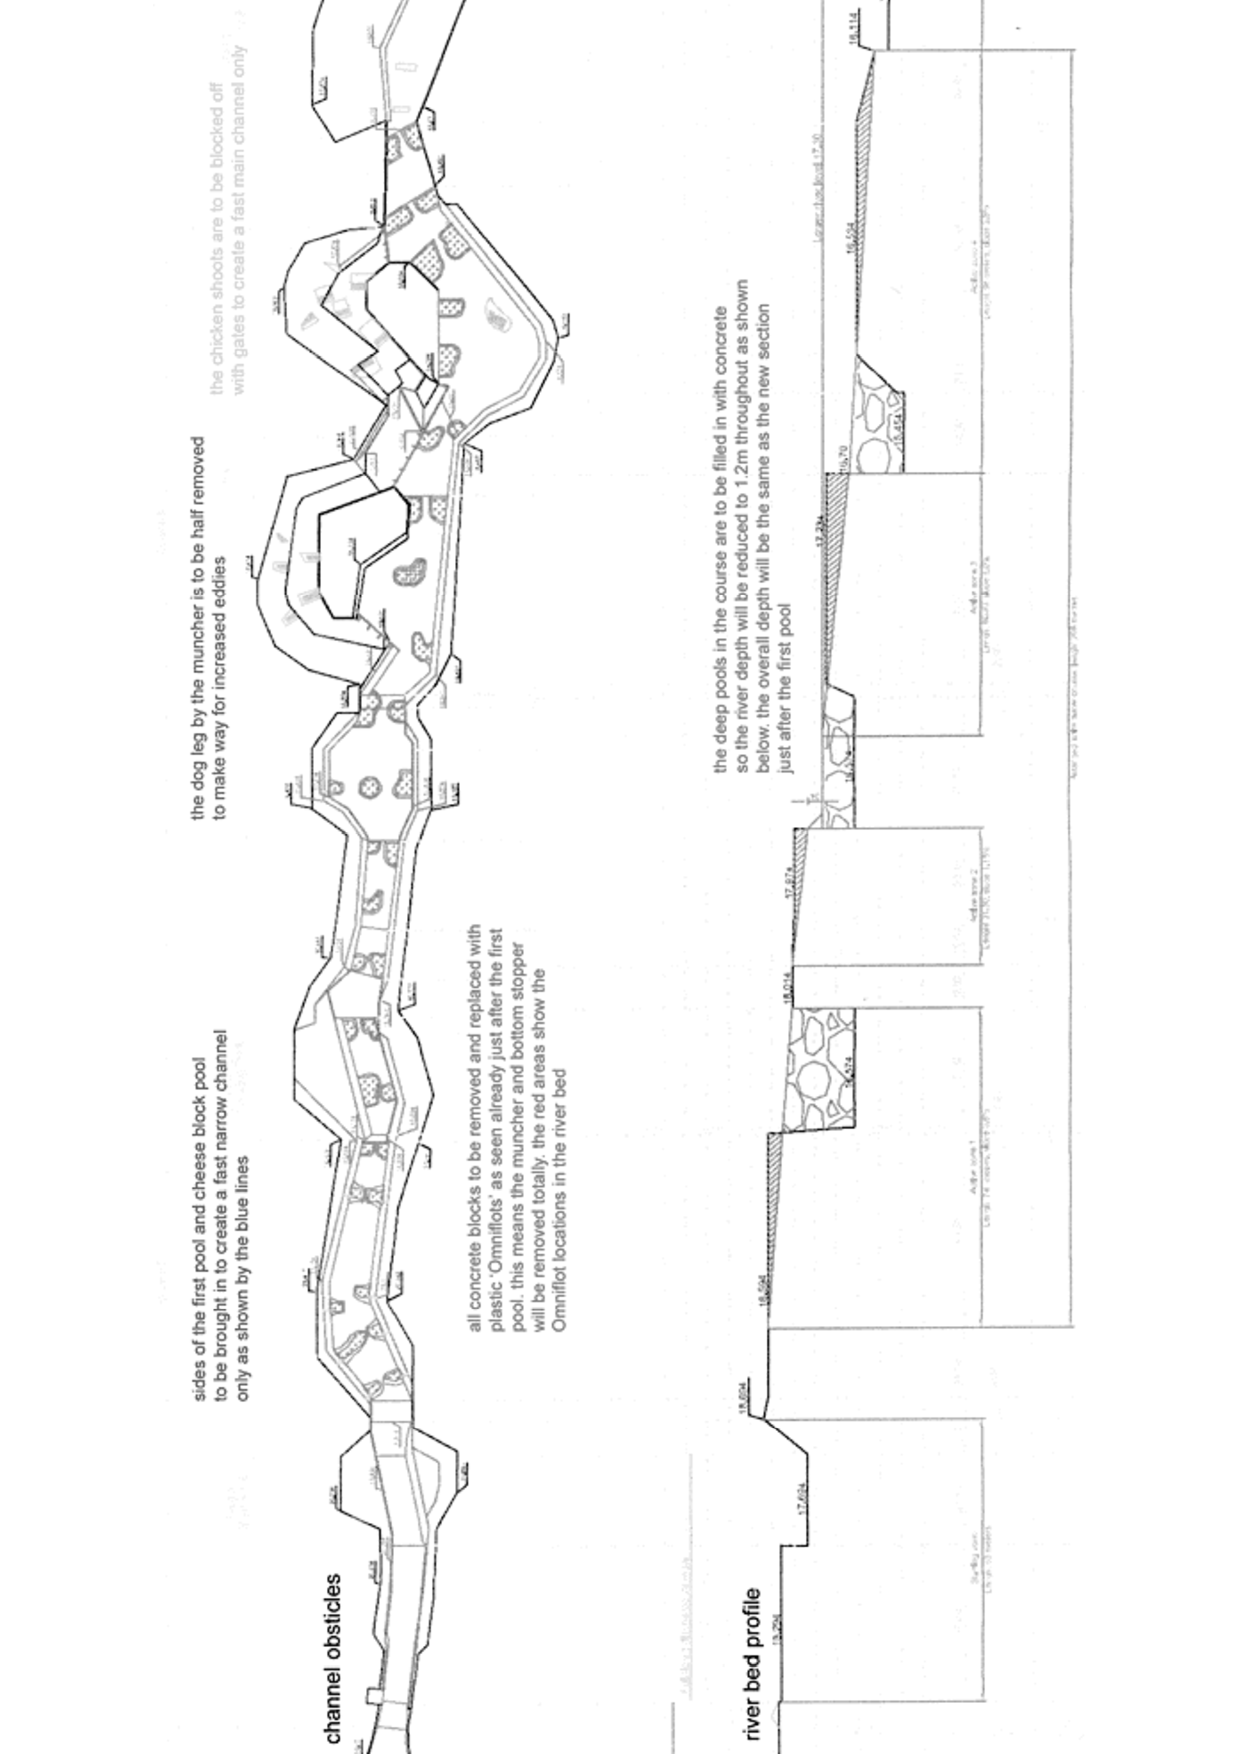
\includegraphics[height=\textwidth,angle=-90]{fig/hpp-plansbw.pdf}}
\caption{\textbf{The proposed plans for the change of the UK National Watersports Centre Whitewater Course (Holme Pierrepont).} Walk based clustering is analogous to the movement of a river. Clusters (or modules) are identified as areas where the `flow' becomes trapped, much like water in the pools immediately following a hydraulic jump. Source: \citep{hpp} }\label{fig:hpp}
\end{figure}

\subsection{Louvain Clustering}

The Louvain clustering algorithm is one of the most popular of the clustering algorithms due to its algorithmic and qualitative robustness, \citep{loudvain,loudrobust}. On the simplest level, this works by maximising the modularity for each configuration. Modularity is a value between positive and negative unity which measures the density of edge between inter and intra communities and compares it to an equivalent random network.
The Louvain is a hierarchical clustering algorithm; this means that after each iteration, all nodes which belong to the same cluster are consolidated to form a new `grouped' item. Inter-cluster links are converted into self-links, and intra-cluster links are updated accordingly.


\subsection{Infomap Clustering }


The Infomap clustering algorithm is a flow-based method which operates on system dynamics rather than structure \citep{mapeqn}. It works by trying to minimise the Huffman code \citep{huffman} - a type of optimal prefix code used for lossless compression in computer science and information theory.
Here the frequency of items is grouped to produce a binary decision tree (\autoref{fig:huff} left). Here the letters a,d,r,g and b appear much more frequently than ! and c. Navigation this binary tree can then be used to produce a Huffman code for each letter (\autoref{fig:huff} right) where letters with a higher frequency have a shorter code length. This method is used within the infomap algorithm to compresses information about the probability of a random walker transitioning between pairs of nodes in a network. Here the prefix of a Huffman code works much like a postcode (City+Areacode, StreetCode ) to identify regions where the walker gets trapped (clusters of high density with a low probability that the walker leaves).

As the number of partitions grows exponentially with the number of nodes\footnote{See `Bell Numbers' - these count the possibles partitions in a set and have root going back to medieval Japan.} it is not possible to apply a brute force approach to find the best number of partitions. Instead, a variation of the Louvain method applies `submodule exploration' which verifies that large modules should not be broken down into smaller ones and `single-node movements` which allow individual nodes to move between modules. These optimisations avoid the situation of too large modules (where each node has a category to itself) or too small where the number of prefix codes is great.


\begin{figure}[H]
  \centering
  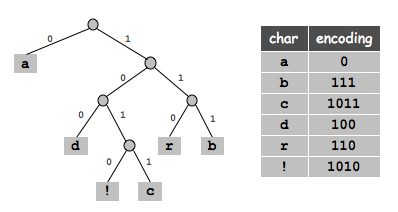
\includegraphics[width=.7\textwidth]{fig/huff.png}
  \caption{\textbf{A Huffman tree, and the Huffman code generated from it.} A Huffman tree is created using the frequency of occurrence of an item. The more often it appears in the source, the shorter the path to it.  Source:\citep{hufftree}}
    \label{fig:huff}
\end{figure}




\section{Selection Criteria For Graph Clustering}

The main two criteria in selecting an algorithm for grouping atmospheric reactions are:

\begin{itemize}
    \item[1.] The algorithm can deal with a directed network - chemistry is directional.
    \item[2.] The algorithm can handle temporal data - The chemistry within a system changes depending on the time of day. This is mainly due to the change in the amount of radiation available from photolytic reactions of oxidants and photolysis reactions.
\end{itemize}

As the InfoMap algorithm implements a directed approach coupled with a multi-level clustering approach able to capture node-layer interaction in temporal networks,\citep{infointermittent}, it makes the right candidate for the task of mechanism reduction.

\section{Evaluation Of Infomap On A Real Simulation.}

Using the initial conditions for London from (\autoref{tab:icsmetric}), a spun up model simulation with the CRI v2.2 mechanism was run. Since this does not contain \ch{c5h11cho}, MVK, MACR or Limonene as primary species, these are omitted from the initialisation. Following a spinup to radical steady-state, a graph is generated for noon after one day of an unconstrained run. The InfoMap algorithm is then applied to the generated graph.

The coarsest level of clustering is shown in \autoref{fig:iml1}. Here nodes are coloured by their cluster, and approximate polygon hulls (a shape of multiple corners which enclose a set of points) surround the nodes closest to the median cluster centre. Much like the findings in (\autoref{ch2}), it is seen that different sections of the graph network represent different types of chemistry - for example, hull 4 contains aromatic species, hull 2 contains the products of linear alkanes and hull 3 contains the terpenes.


\begin{figure}[H]
  \centering
  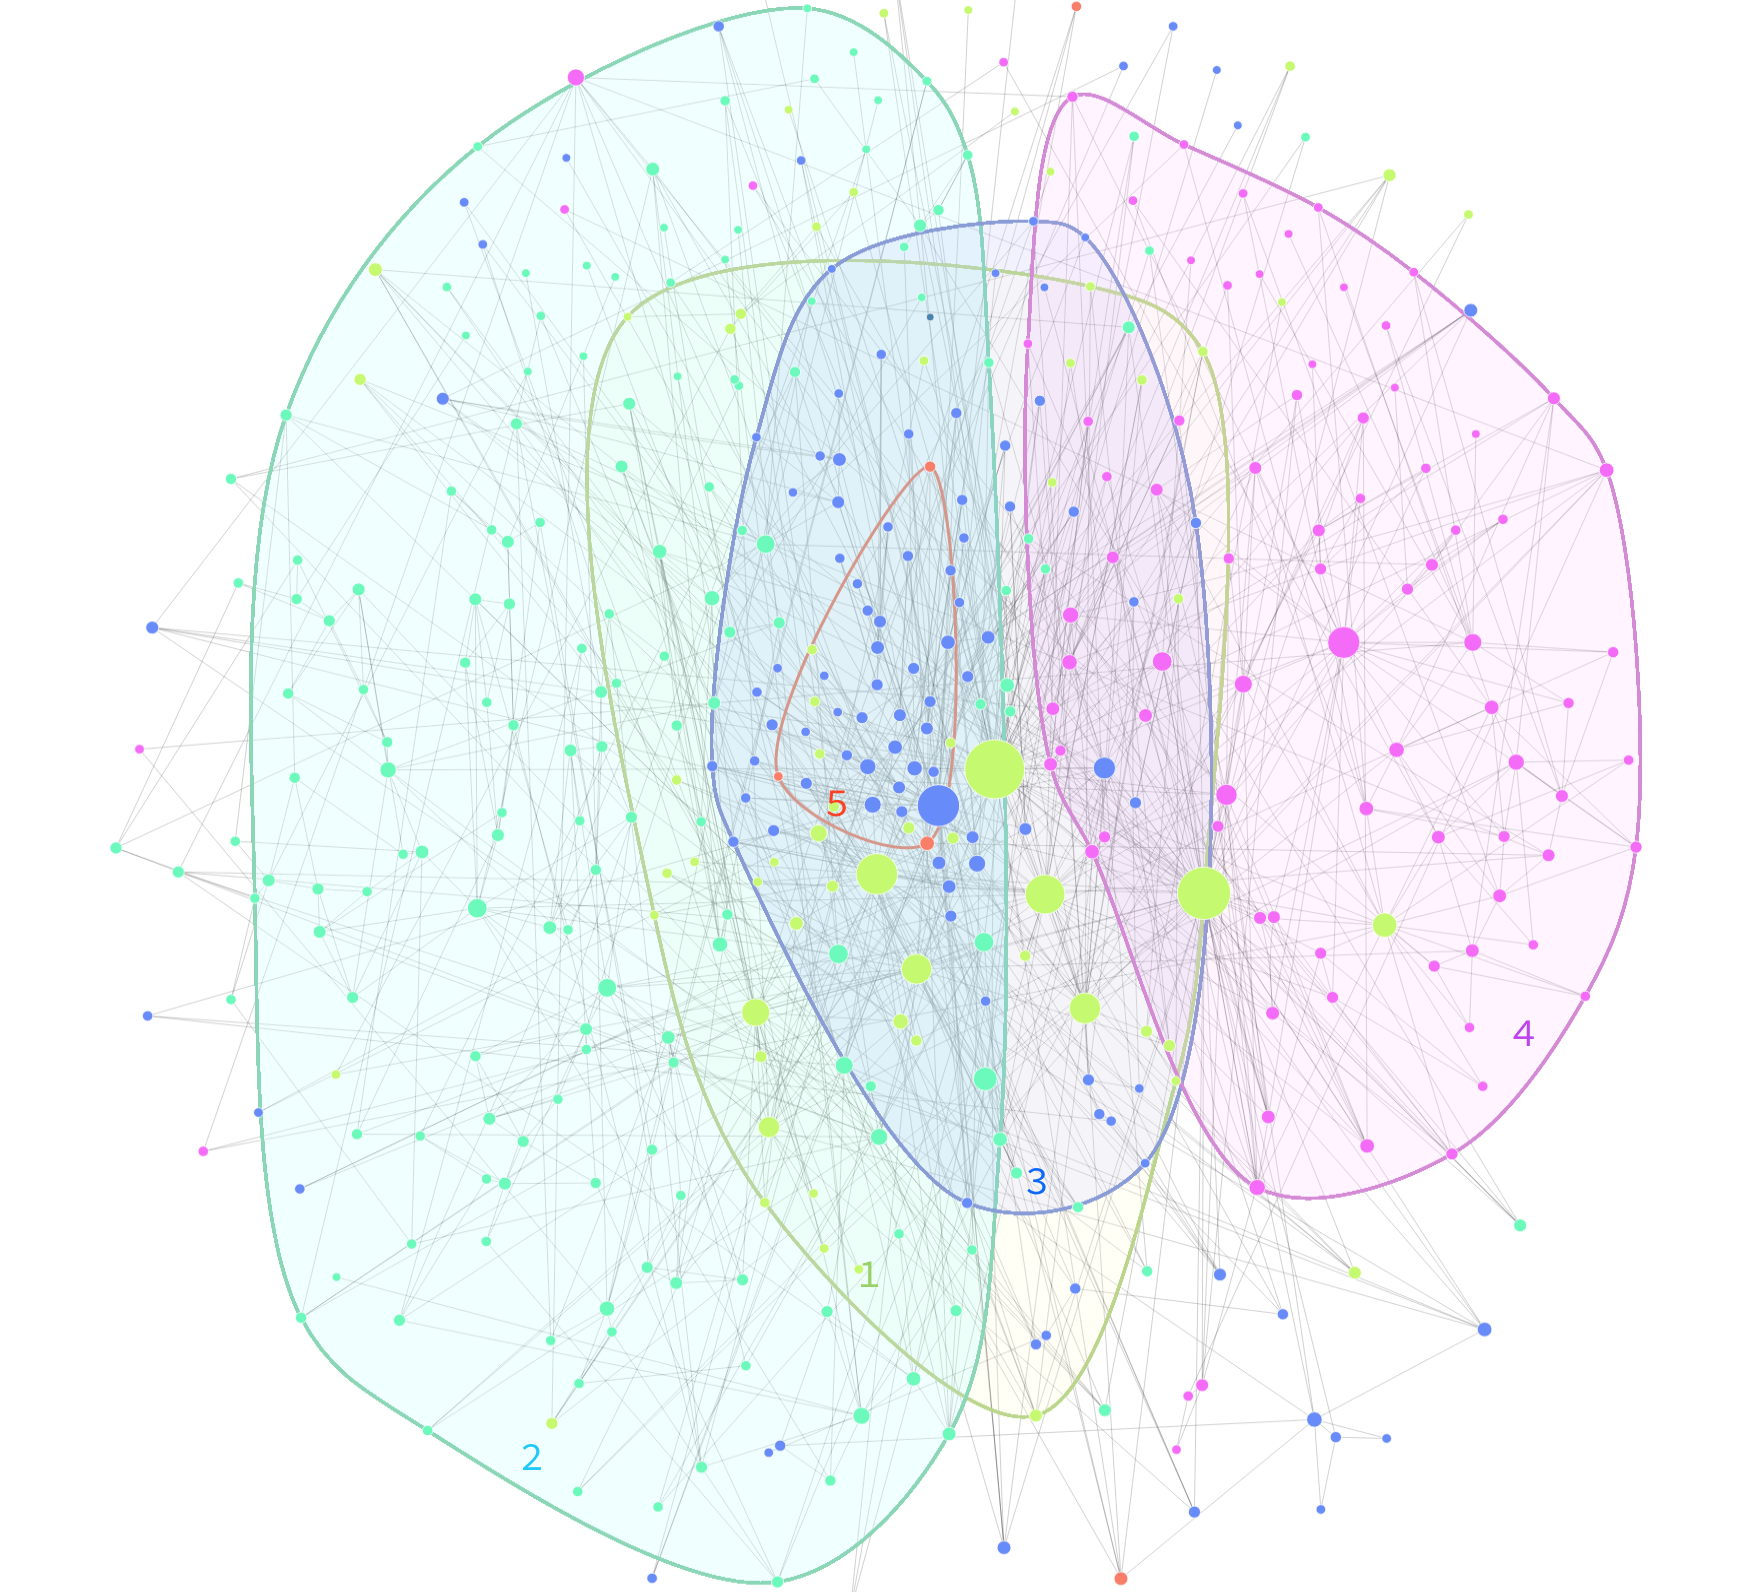
\includegraphics[width=\textwidth]{fig/crigroups.png}
  \caption{\textbf{A graph of CRI v2.2 showing the hulls of the first level of hierarchical clustering.} Nodes are coloured by the splits in branches, and the hulls enclose the nodes which lie within 95\% of the (median) centre of the cluster.}
    \label{fig:iml1}
\end{figure}

As the InfoMap algorithm provides a finer level of clustering, it is essential to evaluate its performance. Using a graph-hull approach, as in \autoref{fig:iml1}, becomes cluttered and unusable. Instead, a bubble plot may be used. Although this sacrifices the ability to view links, it allows for the complete overview of the hierarchical structure. In \autoref{fig:imbubble} shows the nested structure of each clustered group. In an electronic mail correspondence with Mike Jenkin (\autoref{appendix:correspondance}), the origin of the naming convention of reduced species was explained. Individual nodes are coloured by their prefixes. This allows the further categorisation of the species structure within each category.

\begin{figure}[H]
  \centering
  \includegraphics[width=.95\textwidth]{fig/imapbubble.pdf}
  \caption{\textbf{Species structure within each cluster.} A nested bubble chart is used to show the full hierarchical structure of the mechanism. This allows us to evaluate the species structure/type that has been extracted in each level of the hierarchical split. Node sizes are representative of the $\log_{10}$ number of walkers that have become trapped by the flow algorithm at a location. }
    \label{fig:imbubble}
\end{figure}


 \twopagepicture{t}{t}{mechanism_lumping/tree.pdf}{\textbf{A radial treemap showing the hierarchical clustering of the CRI mechanism.} The simulation results used are representative of the chemistry within London at Noon local time and generated using DSMACC and the InfoMap algorithm.
 }{fig:imap2page}{1.0}{0}


\subsection{Species Type And Clustering}
The bubble chart provides an intuitive way to represent groups for interactive or small systems but is less useful for larger numbers of species and print (\autoref{fig:imbubble}). Instead, a tree approach is better suited to revealing the hierarchical structure of the network, as shown in \autoref{fig:imap2page}. Here branches are numerically labelled on each level, allowing us to navigate the structure using a sequence of numbers (e.g. to get to \ch{c4h6} we take the first branch from the centre, followed by the fifth branch after that resulting in the notation 1 . 5 . \ch{c4h6}).

This split notation allows a general overview of the mechanism structure, as well as the reasoning/process of the clustering algorithm. The first level split in \autoref{fig:iml1} shows branches 1,2 and 5 to have origins in the linear (n-) alkane species. This can be seen through both the emitted species (bold) and the \emph{RN} prefix of the species. Here the linear alkanes can react with OH to extract hydrogen and then from a \ce{RO2}, or produce a carbonyl \emph{\ce{CARBxx}}, which can then go on to produce the \emph{\ce{RNxxO2}} peroxy radical.

Except for benzine in 2.14, branches 3 and 4 contain the aromatic species in the network.  Branches 4.\{2,5,9,11\} all consist of \emph{\ce{RAxxO2}} species, which are the product of the addition of OH to toluene/benzine ringed species. 4.\{1,7,8\} and 1.5 contain peroxy radicals formed from the degradation of conjugated dienes \emph{\ce{RUxxO2}}. For the CRI v2.2 mechanism these are only isoprene and 1,3-butadiene. Such peroxy radicals often go on to form unsaturated carbonyls, as denoted by \emph{\ce{UCARBxx}}.

Branch 3 contains the monoterpenes. This can be seen in 3.\{2,5\} ($\alpha-$pinene) and 3.6 ($\beta-$pinenen). Here peroxy radicals formed from the reaction with the e\textbf{n}docyclinc\footnote{Inside the pinene ring.} and e\textbf{x}docyclinc\footnote{Outside the pinene ring.} double bonds of $\alpha-$ and $\beta-$ pinene are denoted with the prefix \emph{\ce{RTN}} and \emph{\ce{RTX}}.

The \emph{\ce{RIxxO2}} prefix was used initially for the peroxy radicals iso (`i-') alkanes and their carbonyl products - branches 3.\{1,4\}, however, they tend to mainly be used for smaller branched precursors which produce acetone (\ch{CH3COCH3}) as a significant product in their oxidation chain (branch 3.1). Acetone is a relatively unreactive carbonyl, the fact that it is water-soluble means that they may be washed out of the atmosphere by precipitation, \citep{acetonerain}. This may have been seen to interrupt the ozone formation process under regional-scale photochemical smog conditions in north-western Europe.

Finally, since the CRI index is representative of the oxidation potential, it is common to see species containing the CRI value within a cluster. Cluster typically contain a combination of carbonyl (\ch{R(=O)R}',\emph{CARBxx}), hydroperoxy (\ch{R-OOH},\emph{RxxOOH}), peroxy (\ch{ROO.}, \emph{\ce{RxxO2}}) and nitrate (\ch{R-ONO2},\emph{\ch{NO3}}) groups. For the lumped species, it can be common for a \ch{RO2} species to react with NO or \ch{NO3} to produce a carbonyl with a CRI index of two values lower. This can be attributed to the loss of hydrogen in the oxidation process. Similarly, a reaction with NO or \ch{ho2} can produce a hydroperoxy or nitrate species, which in turn react with OH to produce the equivalent carbonyl.


%% good paper for introduction acetone
%
% \subsubsection{Inter And Intra Links}
%  Typically, the quality of clustering can be assessed using the adjacency matrix of a graph. In sorting the axis by cluster groups, squares of high-density interconnections should become apparent in an adjacency heatmap. Unfortunately for an atmospheric chemistry mechanism, the size and sparseness of a graph, makes this an infeisable method to visually access the nodcluster node ratios. Instead we can adapt the nodes presented by the treemap in \autoref{fig:imap2page} and replacing the hierarchical structure, with one representing the original graph.
%
%
%    \begin{figure}[H]
%      \centering
%      \includegraphics[width=1.1\textwidth]{fig/treeplot.pdf}
%      \caption{\textbf{The L1 cluster graph using the tree layout from \autoref{fig:imap2page}. } This can be used to explore intra cluster relationships.  }
%          \label{fig:imtreeplot}
%    \end{figure}
%
%



 \subsection{Number Of Clusters}
Sometimes it may be required to have a preset (target) number of clusters. The InfoMap algorithm contains a \emph{preffered number of modules} parameter which can either terminate the algorithm early, should the number be reached (or continue splitting if it has not). Since we are interested in merging smaller numbers of nodes, this can be seen as a useful parameter to have. However, in selecting a number too large, (e.g. 200 clusters, which should result in groups of 2-3 nodes), it is seen that much of the hierarchical information from the network is lost, \autoref{fig:im200}. It is for this reason that forcing the number of nodes without reason will not be attempted.


  \begin{figure}[H]
    \centering
    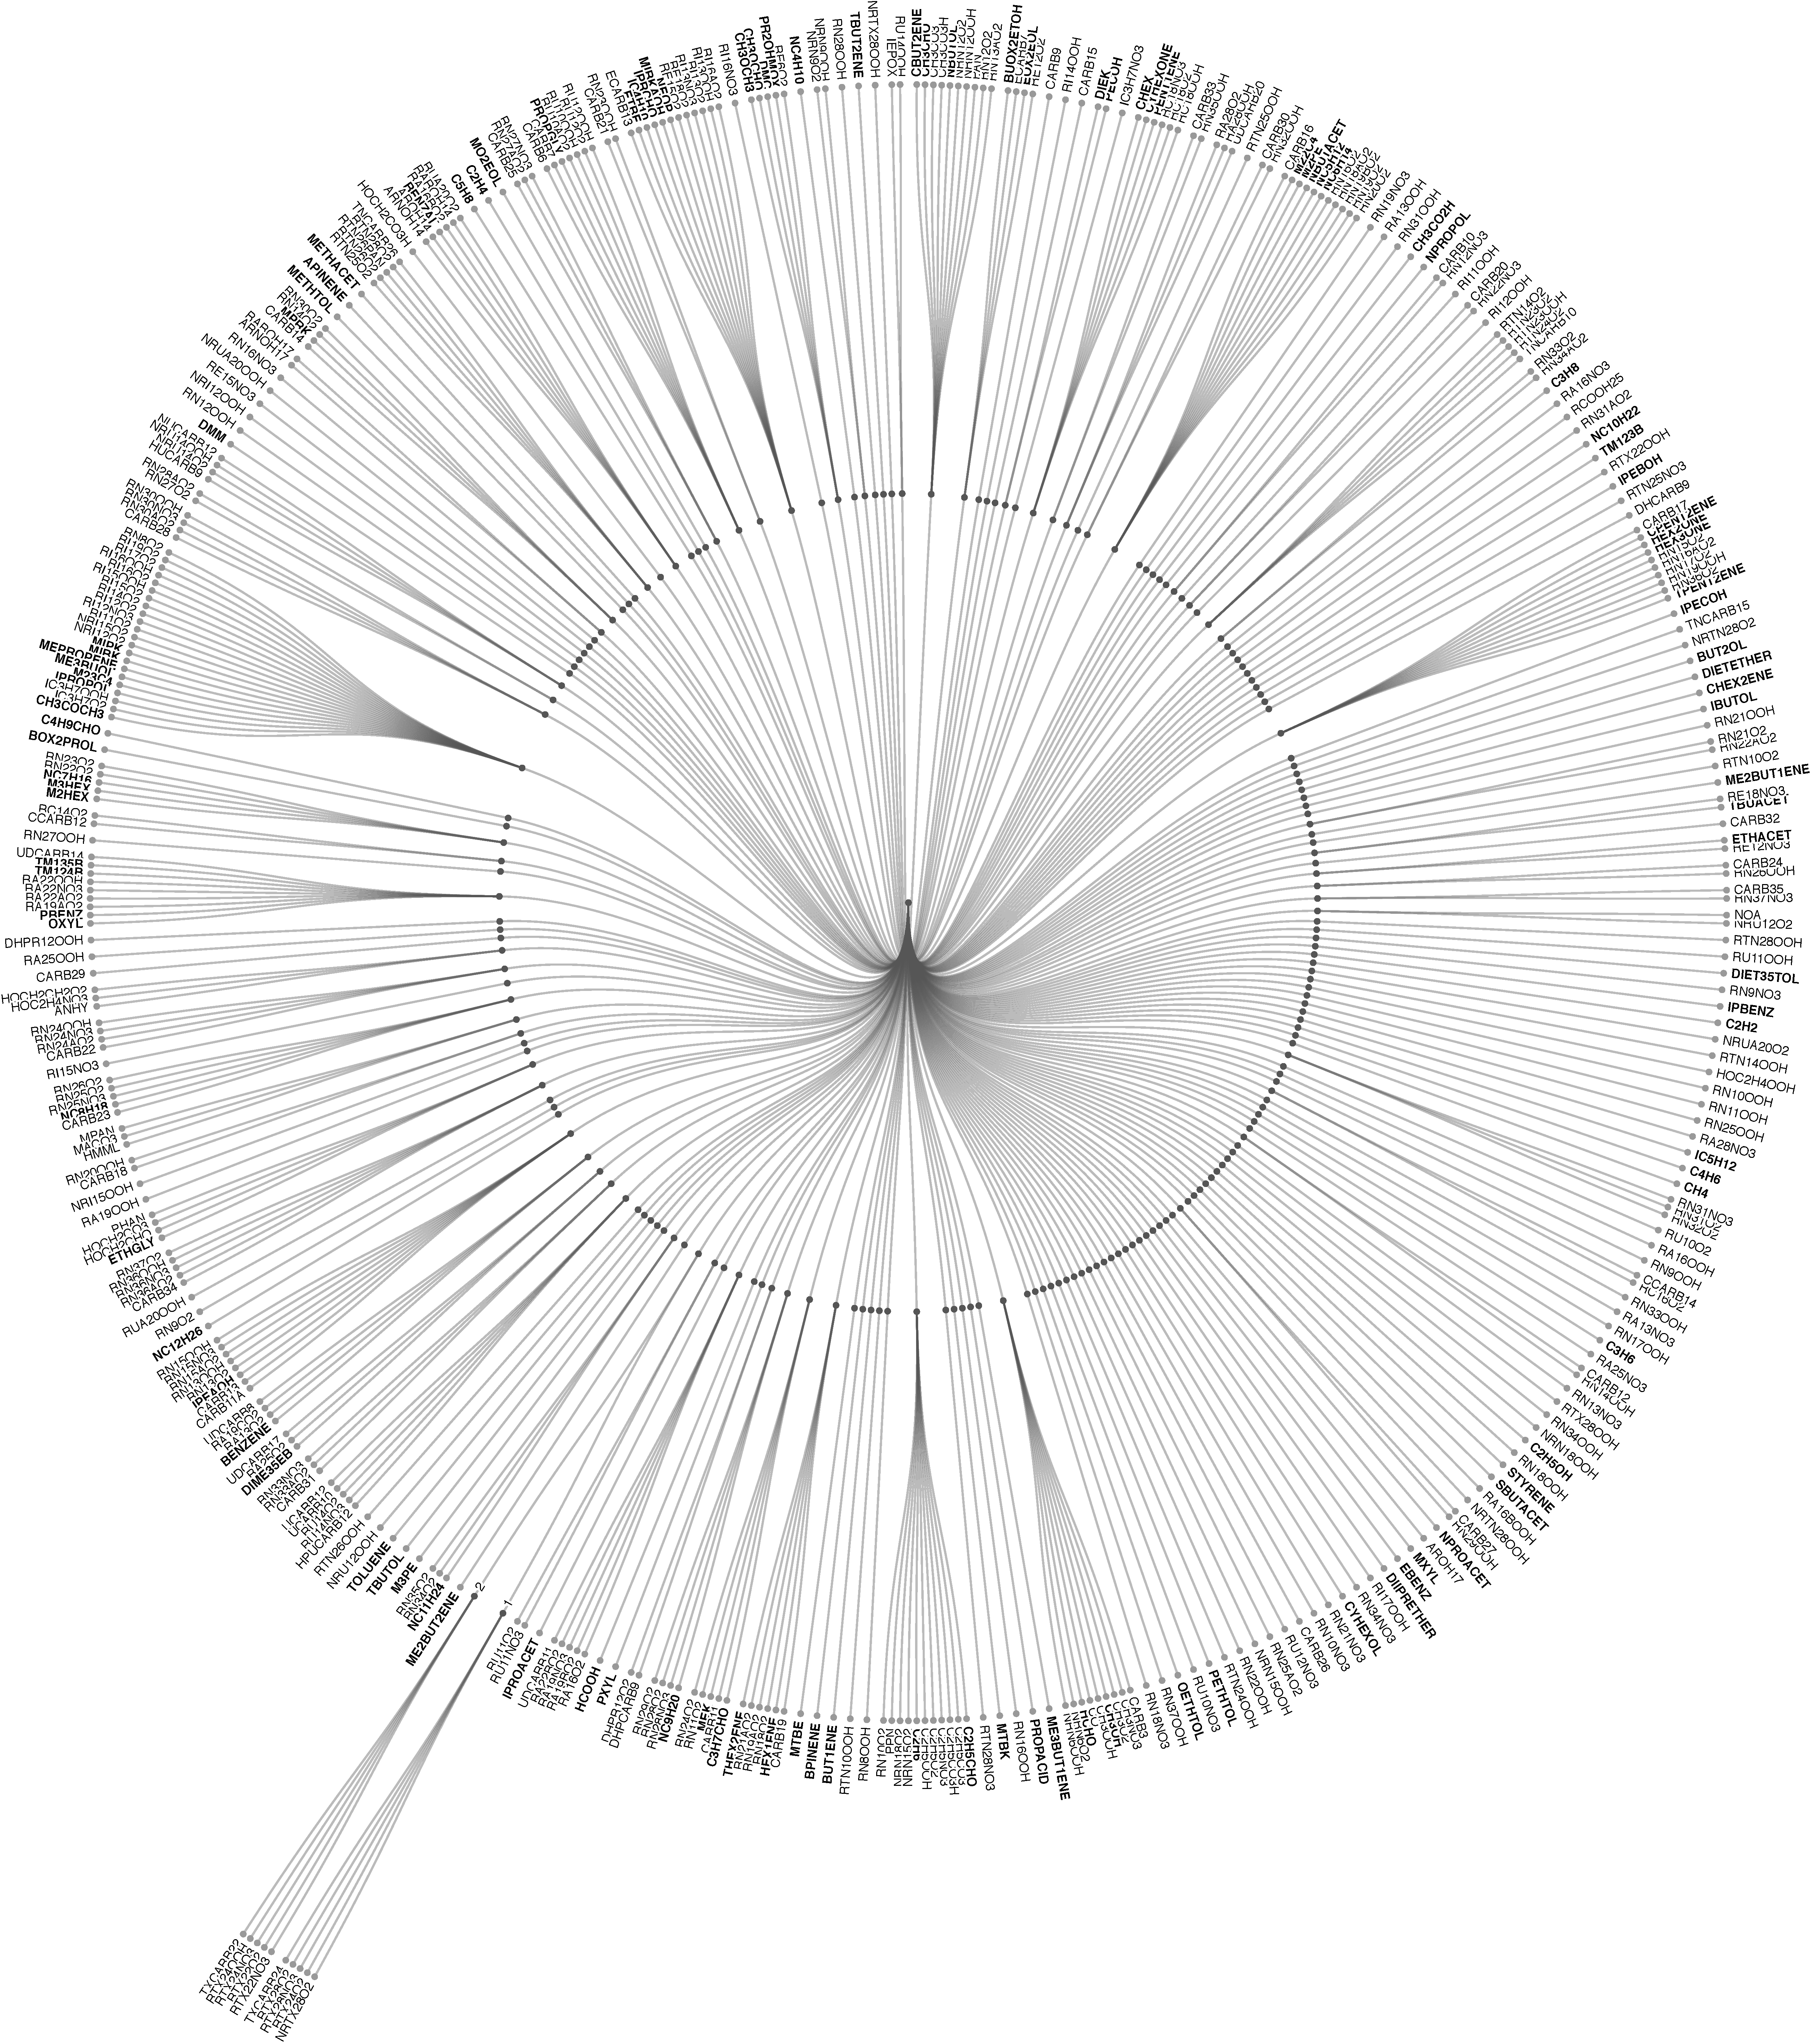
\includegraphics[width=.8\textwidth]{fig/manygroups.pdf}
    \caption{\textbf{A radial tree of the InfoMap algorithm with a forced number of groups.} Here a loss of hierarchical structure can be seen when compared to \autoref{fig:imap2page}. By setting a high number of required clusters, many species are grouped by themselves, which does not provide a useful output for mechanism lumping. }
        \label{fig:im200}
  \end{figure}






  \section{Reduction Through Lifetime}\label{sec:lifetime}
  In \autoref{sec:chemlump} is was mentioned that a species lifetime could be used to decide on which species may be lumped together. Here \cite{lifetime} found that large groups of species within the MCM had similar or identical lifetimes and that in many cases this could be attributed to similar/identical rate coefficients for the same type of reaction. This was then used as a methodology for automatic mechanism reduction.

  This section describes a method in which this may be performed without prior knowledge of the mechanism. Natural language processing tools are applied first to determine species of a similar lifetime across a range of timesteps (\autoref{sec:euclid}), and then their standardised temporal profiles are compared (\autoref{sec:cosine}). However, we first begin by defining the lifetime of a species.

  \subsubsection{Calculating The Lifetime}
  The chemical lifetime is of a species is defined by calculating the lifetime of a species against the loss of individual reactions:





    \begin{equation}
    \tau_A = \frac{1}{\Large{\Sigma}_{i=1,n}\  {1}/{\tau_{A_i}}}
    \end{equation}

where $\tau_A$ is the overall lifetime of species A and $\tau_{A_i}$ are the lifetimes of a die to a loss from reaction 1 to $n$ \citep{fundamentals}. It can be noted that this equation is calculated as part of the diagonal ($J_{ii}$) of the Jacobian matrix \citep{kinetics,lifetime}:


  \begin{equation}
  \tau_A = - \frac{1}{J_{ii}}
  \end{equation}

Where $i$ corresponds to the index of species A in the matrix, since this is a loss, the value of $J_{ii}$ will be negative unless a species does not contain a consuming reaction (then it will be zero).

  %
  %
  % . In chemical simulations, this translates as the time it would take for a species concentration to decrease by two for a case where the production flux of that species is 0, and all rate constants remain constant. For the first-order decay of sample \autoref{eqn}, we can represent the decay using \autoref{decay}. This shows that the half-life of a species is independent of initial concentration.
  %
  % \begin{equation}
  % A \rightarrow[k] B
  % \label{eqn}
  % \end{equation}
  %
  % \begin{equation}
  % s(t) = a_0 \exp(-kt) \\
  % \frac{a(t)}{a_0} = \exp(-kt) \\
  % $$linearised this gives$$
  % \ln (\frac{a(t)}{a_0}) = -kt
  % $$ after $\tau_{1/2}$ the concentration is equal to $a_0/2$ of initial rate $a_0$, which gives $$
  % \ln(\frac{\frac{a_0}{2}}{a_0}) = \ln(\frac{1}{2}) = \ln(2^{-1}) = -\ln2 = k\tau_{1/2}
  % $$$$
  % \tau_{\frac{1}{2}} = \frac{\ln 2}{k}
  % \label{decay}
  % \end{equation}
  %
  % In species of the first order only, this may simplified to
  % \begin{equation}
  % a(t) = a_0 \exp (t  \sum_j k_j )
  % $$ and therefore the half life may be written as the reciprocal sum of rate coefficients: $$
  % \tau_A = 1 / \sum_j k_j
  % \end{equation}
  %
  % and is how lifetime is calculated for photochemical species [ref! modelling book, which references pilling and seakings].



  \subsection{Comparing Magnitude And Direction}
The most significant changes of a reaction rate within a simulation are due to photolytic reactions. Here the solar zenith angle determines the amount of radiation which can reach (and excite) a molecule. Since the chemical lifetime of a species takes into account its loss due to other reaction, such temporal changes in reaction rates need to be taken into account. The simplest method is to construct a vector for each species, showing how their lifetimes change over time. In doing so, we can apply natural language processing techniques, such as euclidean (magnitude) and cosine (angle) distance, co compare them.

  \subsubsection{Euclidian Distance} \label{sec:euclid}
  This is the simplest method of vector comparison and works by calculating the distance between all points in two vectors. For the vectors

  \begin{equation}
  v1 = [ a,b,c, \dots n ]
  $$$$
  v2 = [ i,j,k, \dots z ]
  \end{equation}

  This can be done using pythoagoras' theorem in \autoref{euclid}:

  \begin{equation}
  e_{dist}  = \sqrt{(a-i)^2 + (b-j)^2 + (c-k)^2 + \dots + (n-z)^2}
  \label{euclid}
  \end{equation}

  This transformation converts the straight line distance between each vector into metric space, allowing us to represent the difference in their magnitudes as a single scalar. Unfortunately, as this requires the difference between all permutations of rows, it cannot be done as a single operation.

  \subsubsection{Cosine Distance}\label{sec:cosine}
  Similar to euclidean distance, if we wish to calculate the angle between two vectors, we may use the cosine difference. In starting with the definition of the dot product

  \begin{equation}
  v1 \cdot v2 = \|v1\|\|v2\| \cos \theta
  $$this may be arranged$$
  \cos \theta = \frac{ v1 \cdot v2}{\|v1\|\|v2\|}
  \end{equation}

  The problem is that for a meaningful representation for the cosine inequality, the Cauchy-Schwarz (triangle) inequality needs to be satisfied. This states that for all sequences of real numbers $a_i$ and $b_i$:

  \begin{equation}
      (\Sigma a^2_i)(\Sigma b^2_i) \ge (\Sigma a_ib_i)^2
  \end{equation}

  Each vector needs to be normalised before the calculation of the angle. This eliminates information about the magnitude of the vectors but also allows for a better comparison of the distribution (or shape). This normalisation factor makes it particularly useful in the analysis of text documents, where a word may appear multiple times in different length segments.



  \subsection{Temporal Lifetime Vector Comparison}

  To compare a species diurnal profile with its absolute lifetime, we can plot the cosine and euclidian distance against each other on a $x-y$ scatterplot, \autoref{fig:metric}. In this subsection, we compute the Euclidean and cosine distances for all remaining reaction pairs (88410 pairs) for a single simulation from the setup described in \autoref{sec:lumpinputs}. We start by looking at the species density profiles, \autoref{fig:density2}.




  \begin{figure}[H]
  \begin{subfigure}[t]{.5\textwidth}
    \centering
    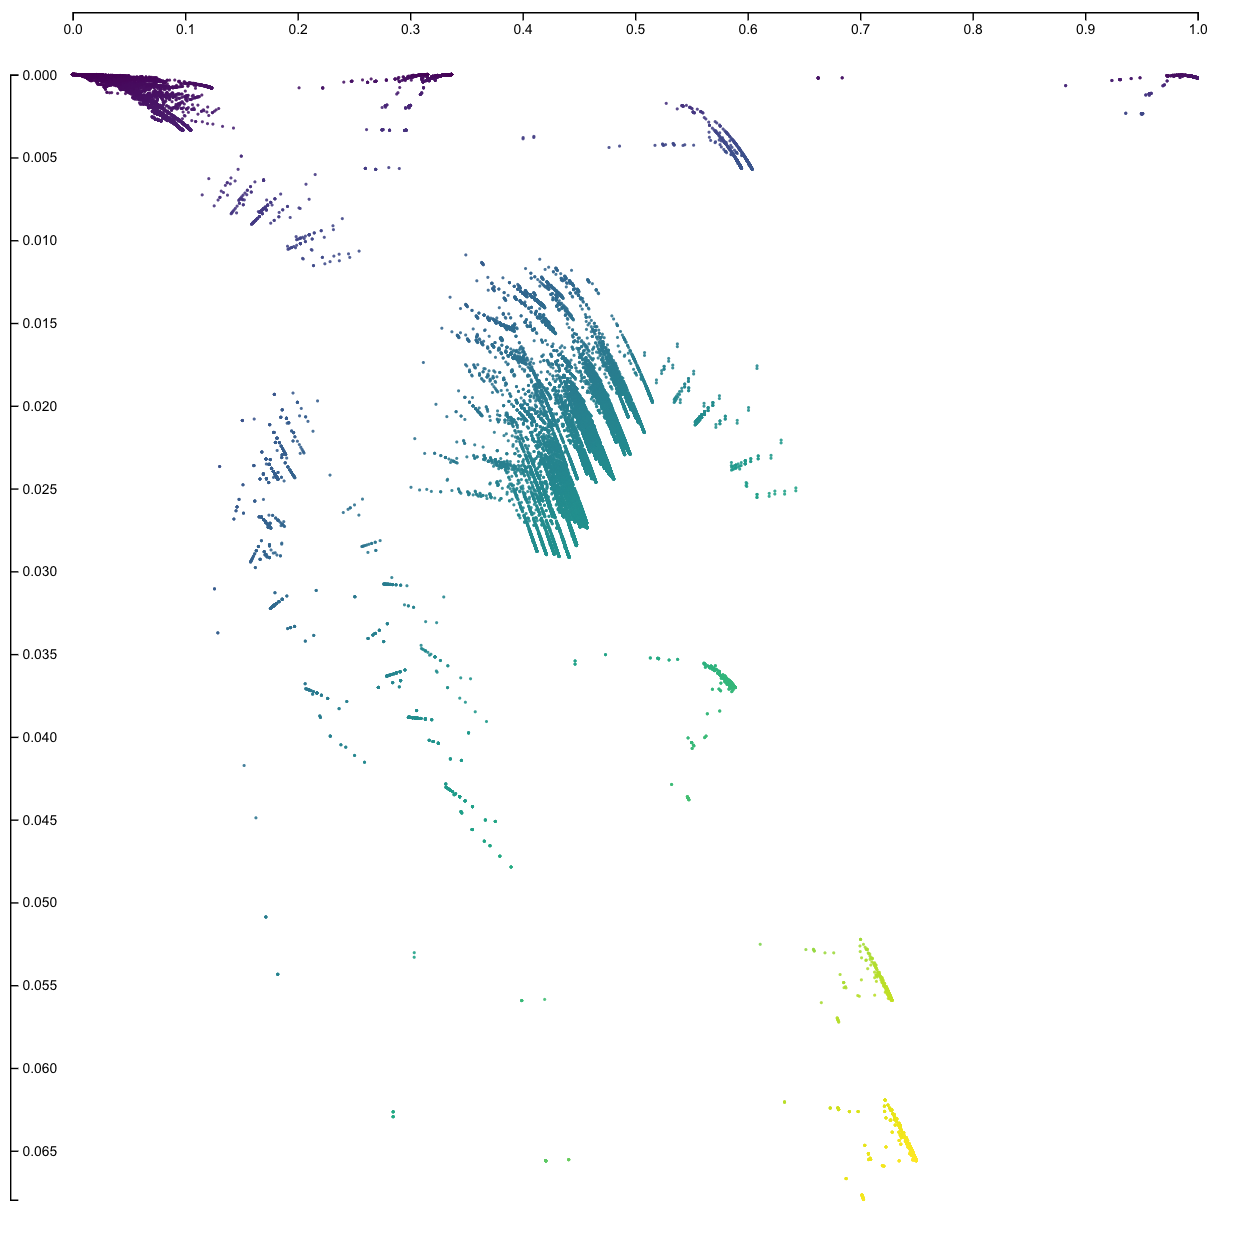
\includegraphics[width=\textwidth]{fig/metric-1.png}
    \caption{Original}
    \label{fig:morig}
  \end{subfigure}%
  \begin{subfigure}[t]{.5\textwidth}
  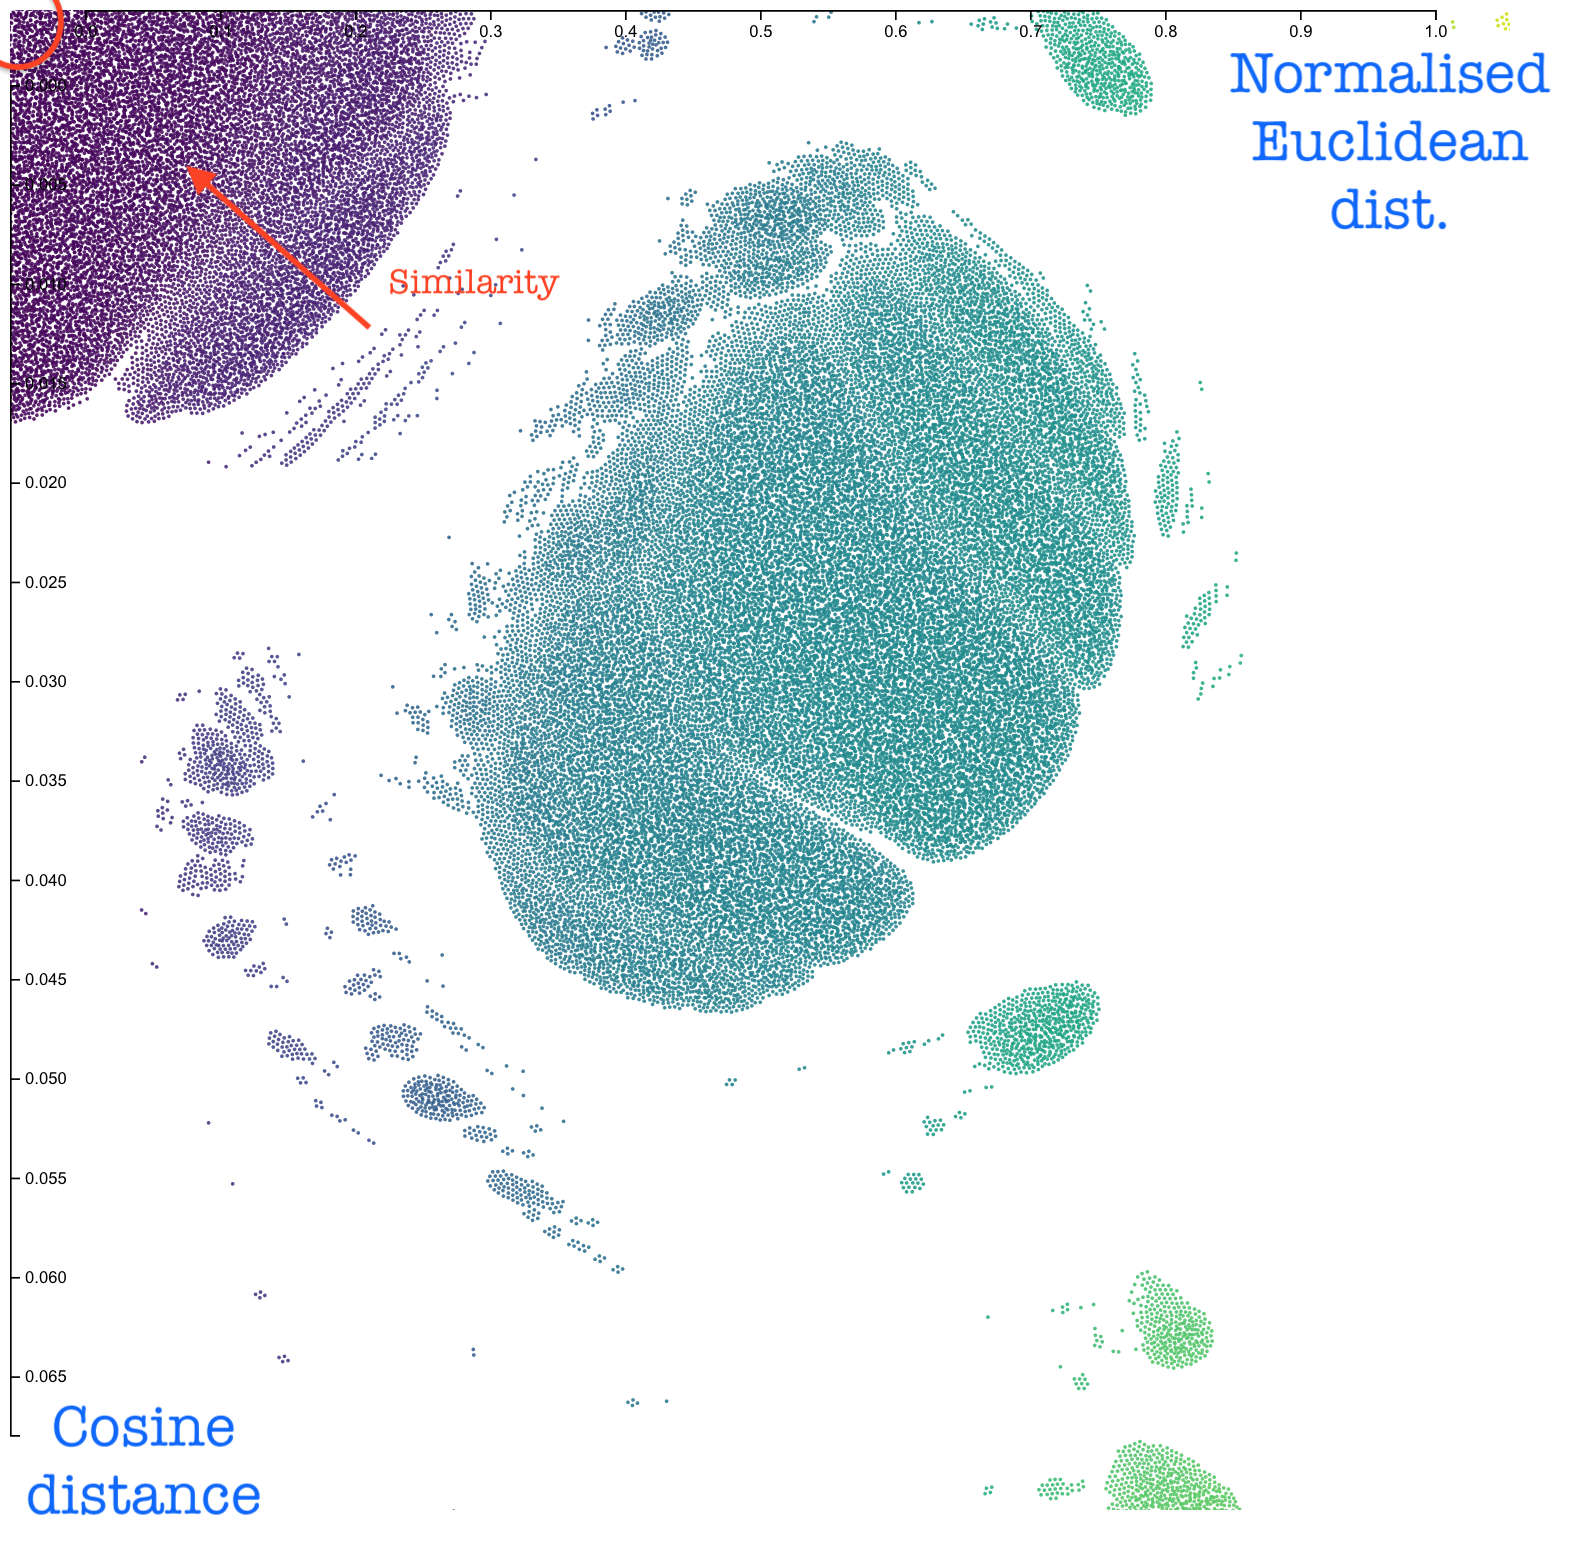
\includegraphics[width=\textwidth]{fig/metric.png}
  \caption{No-overlap}
  \label{fig:metric}
  \end{subfigure}
  \caption{\textbf{Cosine distance against Euclidian Distance}. Normalised version of the two distance metrics are plotted in an $x-y$ scatterplot. Each dot represents a different species pair plotted at the location of their value for each metrics. Species pairs with similar values and profiles have small values for each metric and are located towards the upper left hand corner. (b) shows the same results as (a) but has a no-overlapping (collision detection) algorithm applied show all points, and therefore aid interactive selection.}
  \end{figure}


  \textit{NOTE: the kernel density plot $x$ axis shows 1-(the value shown in the scatter plot). This is because output values from each distance closer to 1 are similar. In the scatter plot inverting this however proved more straightforward to plot and explain}


  Similar to \cite{lifetime}, we find there are several groups of species with similar lifetimes. In general, we have two main peaks where the temporal profile and concentration differences are similar. Here the first peak (\autoref{fig:density2} from the right) shows a significant agreement between both similarities. This suggests that most of the species within this section react similarly, and will very likely have the same inorganic reactions at a similar rate. The second peak, however, shows species which have a similar diurnal response, with different magnitude differences. These species are likely affected by photolysis reactions directly or indirectly but have a differing set of reactions controlling them. In a concentration line-plot we would expect them to have peaks in the same location, but to change at a different rate/magnitude to each other.


  \begin{figure}[H]
      \centering
  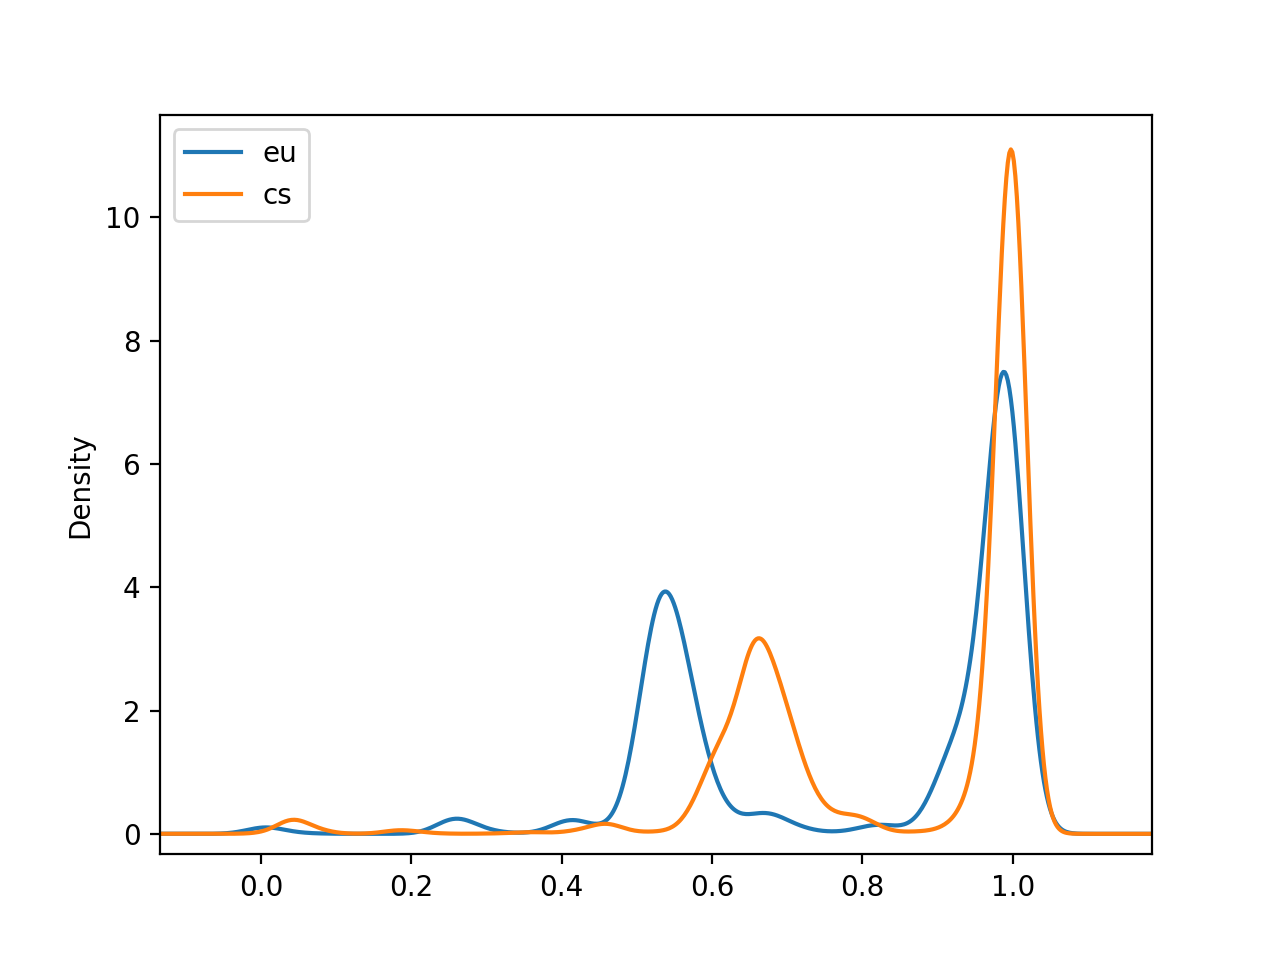
\includegraphics[width=.7\textwidth]{fig/metric_density.png}
  \caption{\textbf{Gaussian Kernel Density Estimate plot showing the distributions present for the \{0,1\} scaled euclidean and cosine distances.} This graph shows the density profiles for each metric in \autoref{fig:morig} - these show 1-(normalised metric distance), and therefore the peak at 1 corresponds to that in the top left of \autoref{fig:morig}. Peaks here correspond to the regions of high densitry within the scatterplot \autoref{fig:metric}.}
  \label{fig:density2}
  \end{figure}



  A comparison of both similarities on the $x-y$ plot is shown in \autoref{fig:morig}. As many species have similar lifetimes, these are often situated within the same temporal space, which can make it hard to visually or interactively separate them. It is possible to convert the scatter plot into a force-simulation, \autoref{fig:metric}. Here nodes repulse each other and are attracted to their original location. This expands the graph and prevents overlapping nodes. In doing so, it is possible to interactively query the pairs of nodes which are represented by each point if required. This information can be better shown in a Kernel density plot comparing the distribution of cosine and euclidean distances.

   The agreement of both metrics suggests a similarity between the lifetime values and their change in time for simulation. This is in agreement of with the $x-y$ plot of the species. In selecting species that are part of the same initial cluster and have a high agreement between both similarities, it is possible to gauge the suitability for two species to be lumped together.


  \subsection{A Quick Concentration Comparison}
  Having described how the similarity distances work, \autoref{fig:metric} showed the locations of the best and worst matched pairs. This subsection looks a the differences between these using a log10 ensemble of the concentrations for the 300 simulations used in the results section. \autoref{fig:bestworst}(a,b) show that the best matching pairs contain an easy to match flat decay curve, with the worst \autoref{fig:bestworst}(c,d) often containing a combination of a species which decays with one which undergoes a photolytic reaction.


  \begin{figure}[H]
  \begin{subfigure}[t]{.5\textwidth}
    \centering
    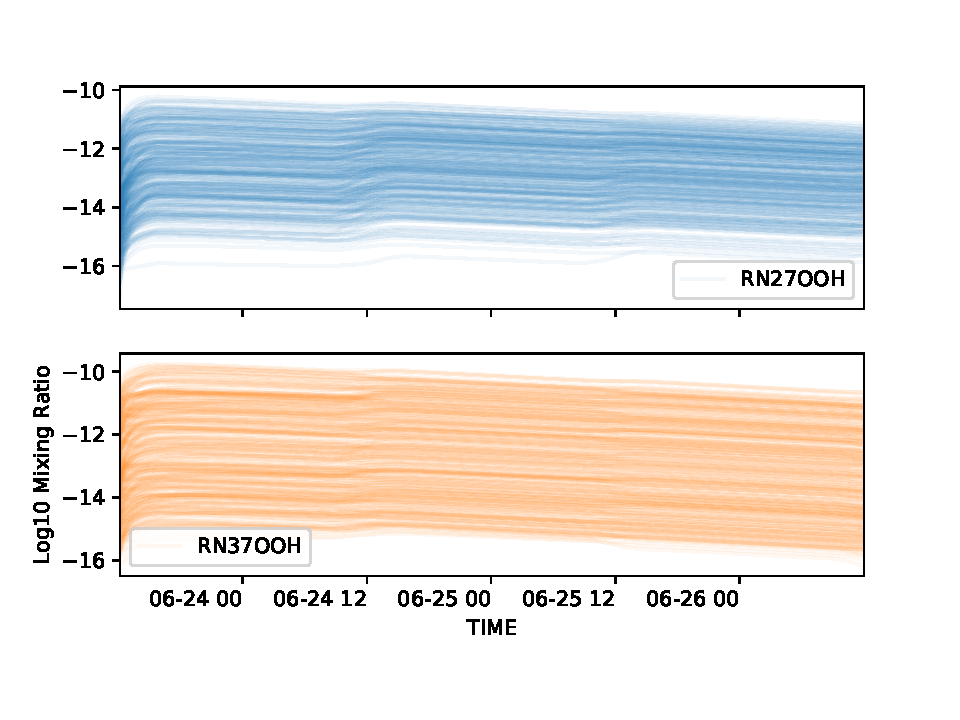
\includegraphics[width=\textwidth]{ensemble/RN27OOH-RN37OOH.pdf}
    \caption{}
  \end{subfigure}%
  \begin{subfigure}[t]{.5\textwidth}
    \centering
    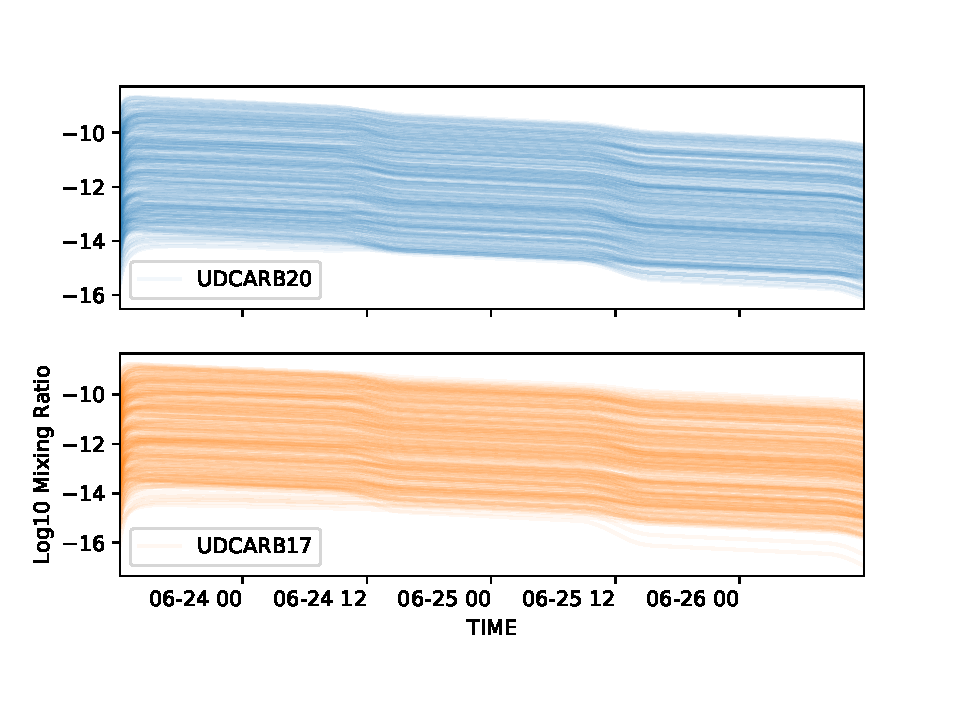
\includegraphics[width=\textwidth]{ensemble/UDCARB20-UDCARB17.pdf}
    \caption{}
  \end{subfigure}%\\

  \begin{subfigure}[t]{.5\textwidth}
    \centering
    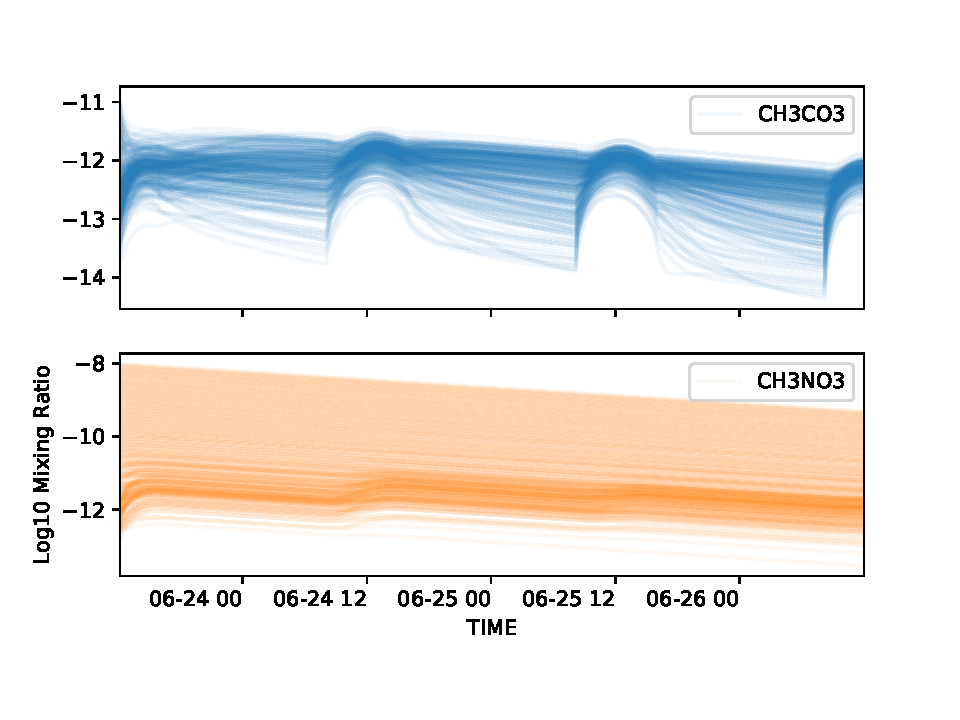
\includegraphics[width=\textwidth]{ensemble/CH3CO3-CH3NO3.pdf}
    \caption{}
  \end{subfigure}%
  \begin{subfigure}[t]{.5\textwidth}
    \centering
    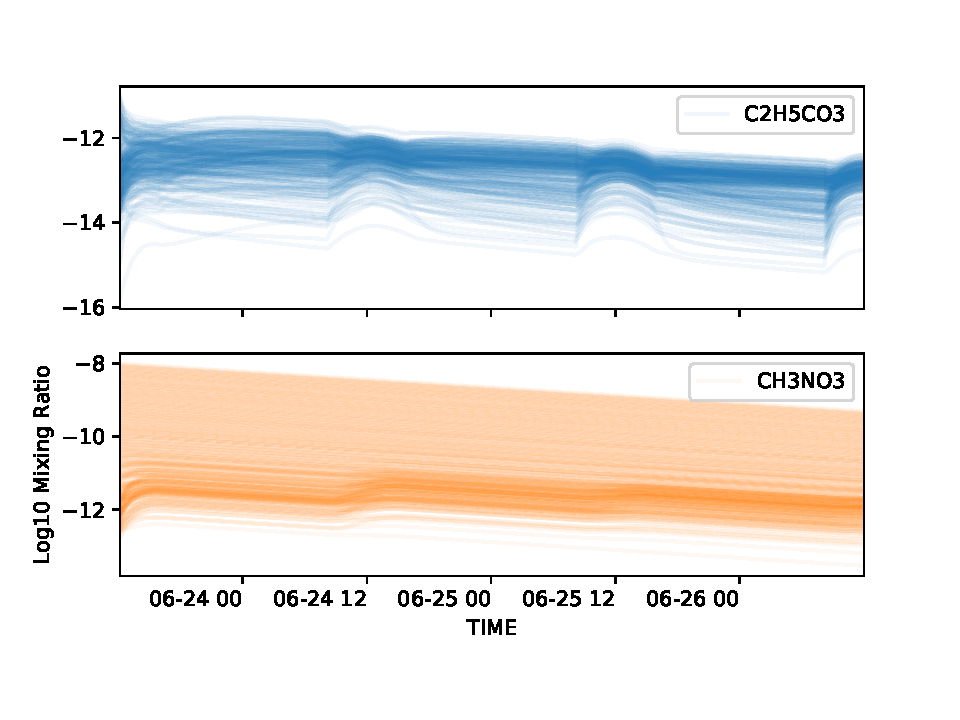
\includegraphics[width=\textwidth]{ensemble/C2H5CO3-CH3NO3.pdf}
    \caption{}
  \end{subfigure}%\\
  \caption{\textbf{Comparing the best (a-b) and worst (c-d) species combinations using the combigned similarity metrics.}Here species which only undergo a simple decay seem to be the easiest to group together. Species pairs between an photolytic and non photolytic species produce different profiles at differing magnitudes and are therefore difficult to match.}
  \label{fig:bestworst}
  \end{figure}






%


\section{Results}

In order to get a representation of the mechanism, we run 300 randomly initiated scenarios (\autoref{sec:lumpinputs}). The experimental setup is one such that it is possible to add more data points at a later date. From each simulation, the no diagonal elements of the jacobian are used to construct a graph representative of the aggregated hourly means of the simulation output. Each of these graphs is then run through the infomap algorithm, and a grouping/clustering produced. Each infomap is run 100 times, where the result with the best fit (shortest code length) is taken - this is an optional parameter on the algorithm.

\subsection{The Co-Grouping Network}

To aggregate the groupings produced by each algorithm an $n\times n$ matrix is created for each of the ($n$) species in the mechanism. This is treated as a relational graph matrix. If species A is in the same group as species B, then a link (or value +1) is added to the [A,B] (A\ce{->}B) and [B,A] (B\ce{->}A) column. Using this matrix format, it is possible to generate a graph showing the relationship between species that were clustered in the same group.

This relational matrix can then easily be converted into the network format: \autoref{fig:infomapprune}a. Starting with this it is then possible to filter edges below a certain weight, \autoref{fig:infomapprune}b-d. Finally, isolates (nodes with no links) are removed, leaving only those clusters where each species has a strong relationship between every other.

In the context of this section, we select only relationships that appear in over 45\% of all the clustered simulation runs. The reasoning is that there may exist a pairing which only appears during day or night time.

\begin{figure}[H]
\begin{subfigure}[t]{.5\textwidth}
  \centering
  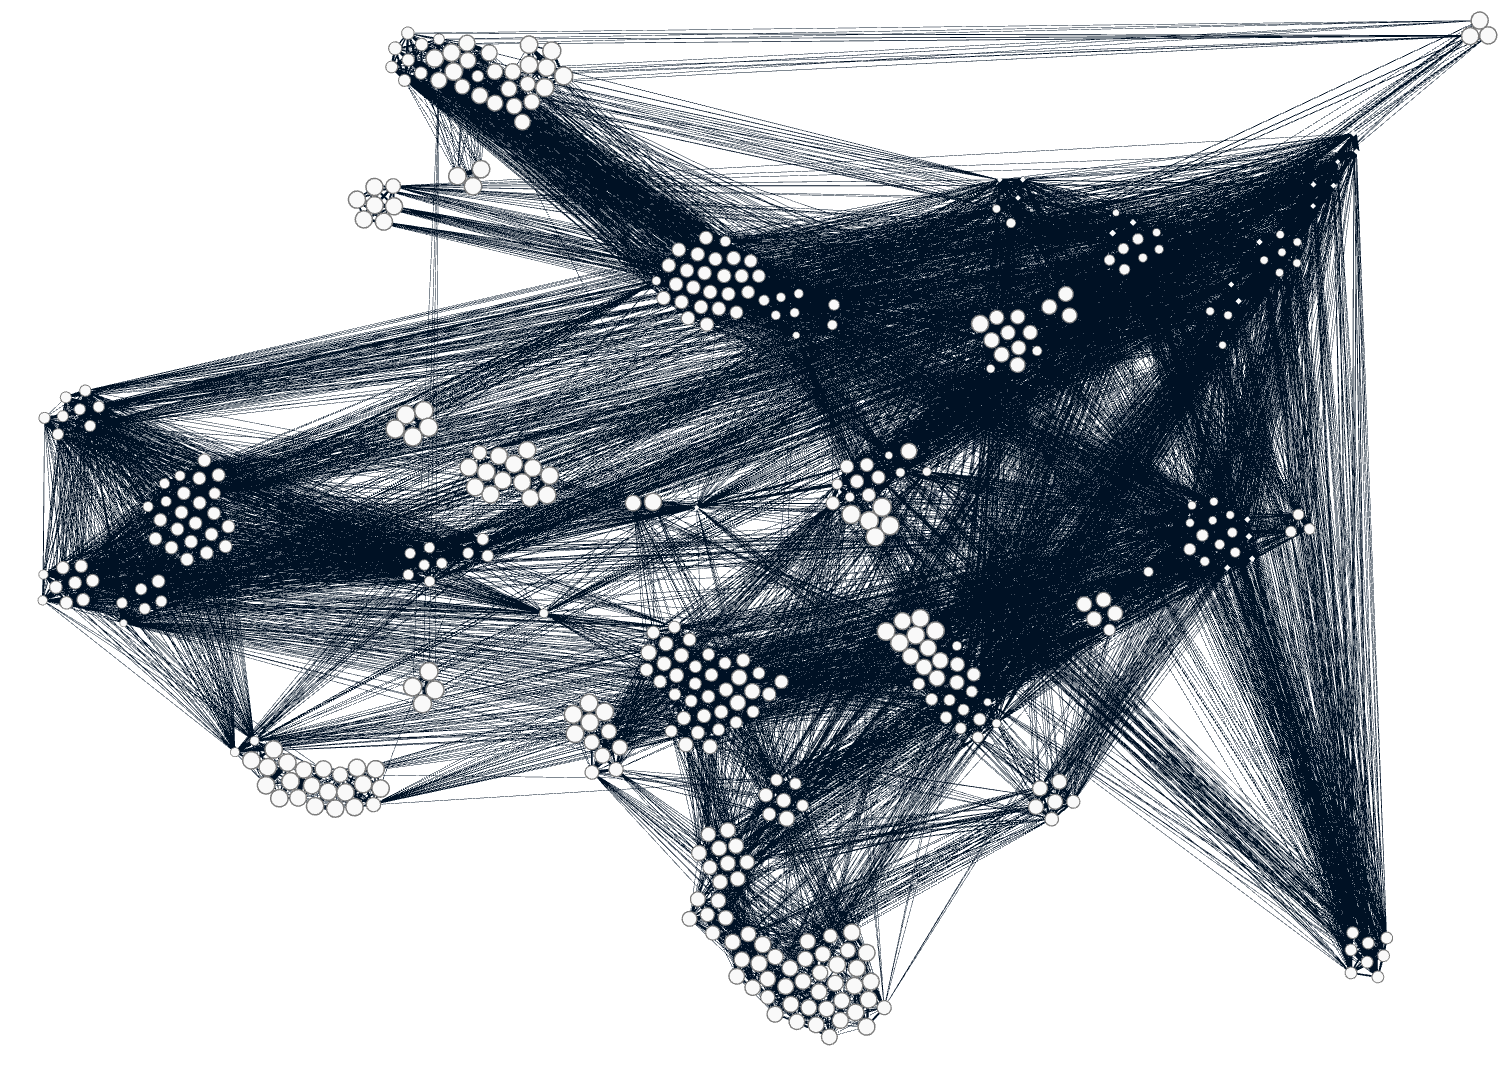
\includegraphics[width=\textwidth]{fig/c1.png}
  \caption{Full Graph}
\end{subfigure}%
\begin{subfigure}[t]{.5\textwidth}
  \centering
  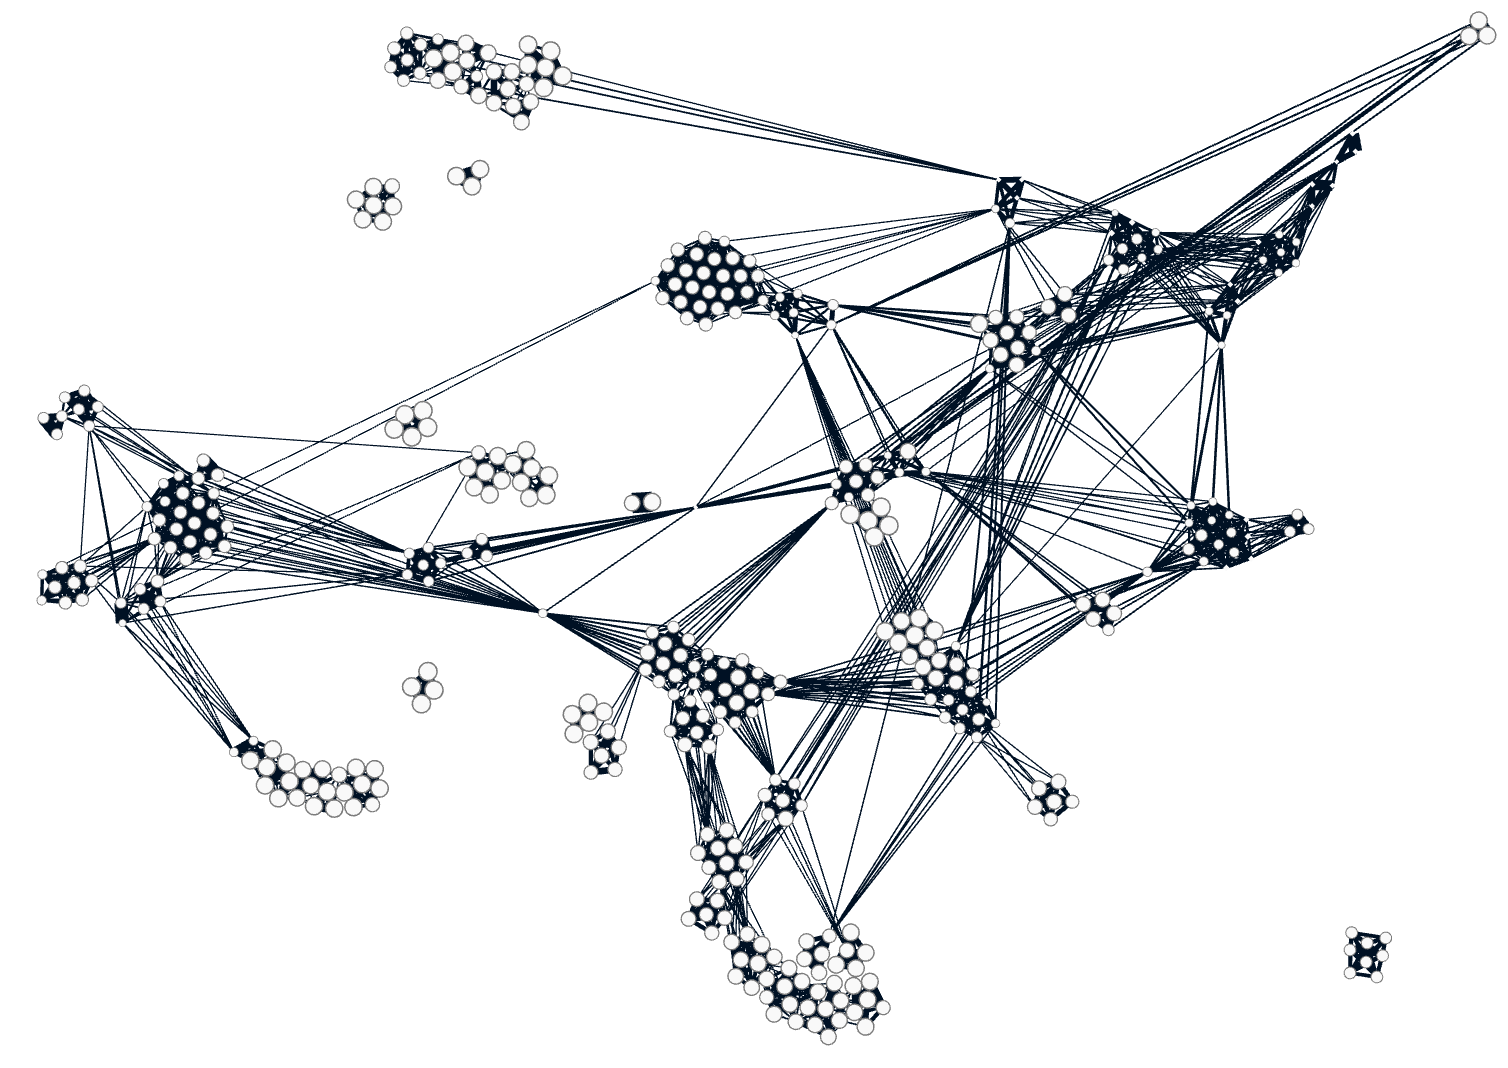
\includegraphics[width=\textwidth]{fig/c2.png}
  \caption{>10\% of graphs}
\end{subfigure}%\\

\begin{subfigure}[t]{.5\textwidth}
  \centering
  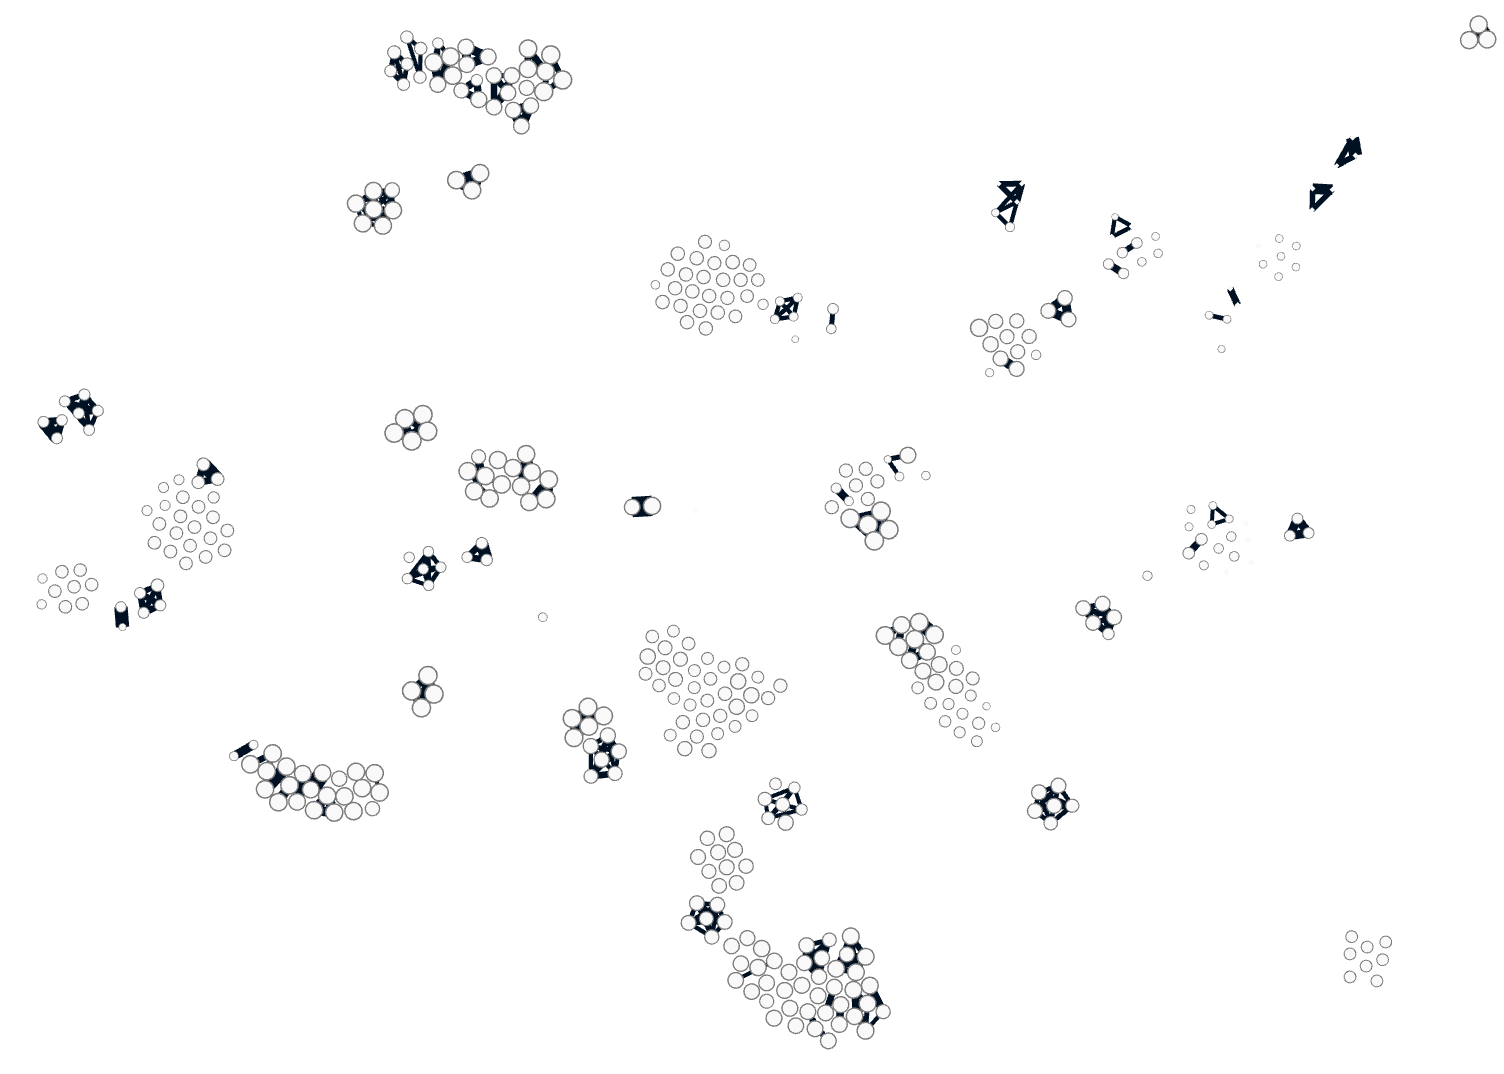
\includegraphics[width=\textwidth]{fig/c3.png}
  \caption{>20\% of graphs}
\end{subfigure}%
\begin{subfigure}[t]{.5\textwidth}
  \centering
  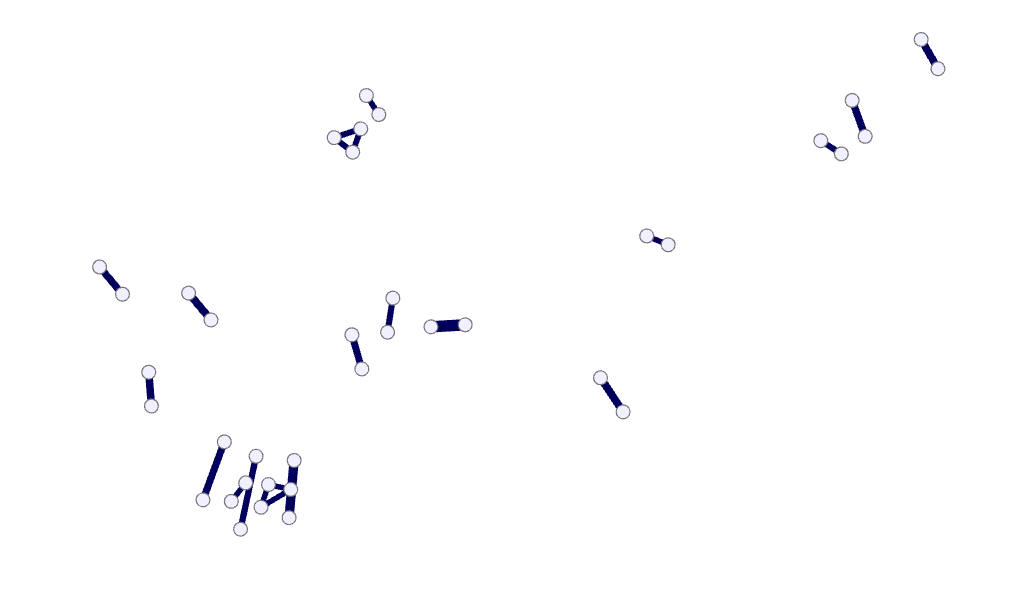
\includegraphics[width=\textwidth]{fig/c4.png}
  \caption{>40\% of graphs}
\end{subfigure}%
\caption{\textbf{Filetering the infomap clustering relationship matrix/graph} How the clustering relationship network changes as weak links (links between species which do not appear in many of the infomap groupings) are removed. }
\label{fig:infomapprune}
\end{figure}

\subsection{Comparing Daytime And Nighttime Groups}
In determining a group of species which are commonly clustered together in most simulation results, we are next interested in seeing if these groups change with day or night.

To do this, we use an alluvial diagram \citep{alluvial}. This is a cross between a parallel-line plot and a Sankey diagram and is particularly suitable for showing the changes in clusters within a temporal network.

In taking the common clusters formed at midnight (\autoref{fig:alluvial} left)  and midday (\autoref{fig:alluvial} right) we are able to compare these to the overall selection (all hours - middle). Here, as is expected, any parings which persist in over 45\% of all the timesteps, exist in all three categories. We see a selection of species which are grouped at 12:00 and 0:00 hours. This suggests that they may not be grouped with some of the intermediate hours and that if the threshold of selection is lowered below 45, they may appear in the overall result—finally a selection of species which are only grouped in daytime or night time only results.



\begin{figure}%[H]
    \centering
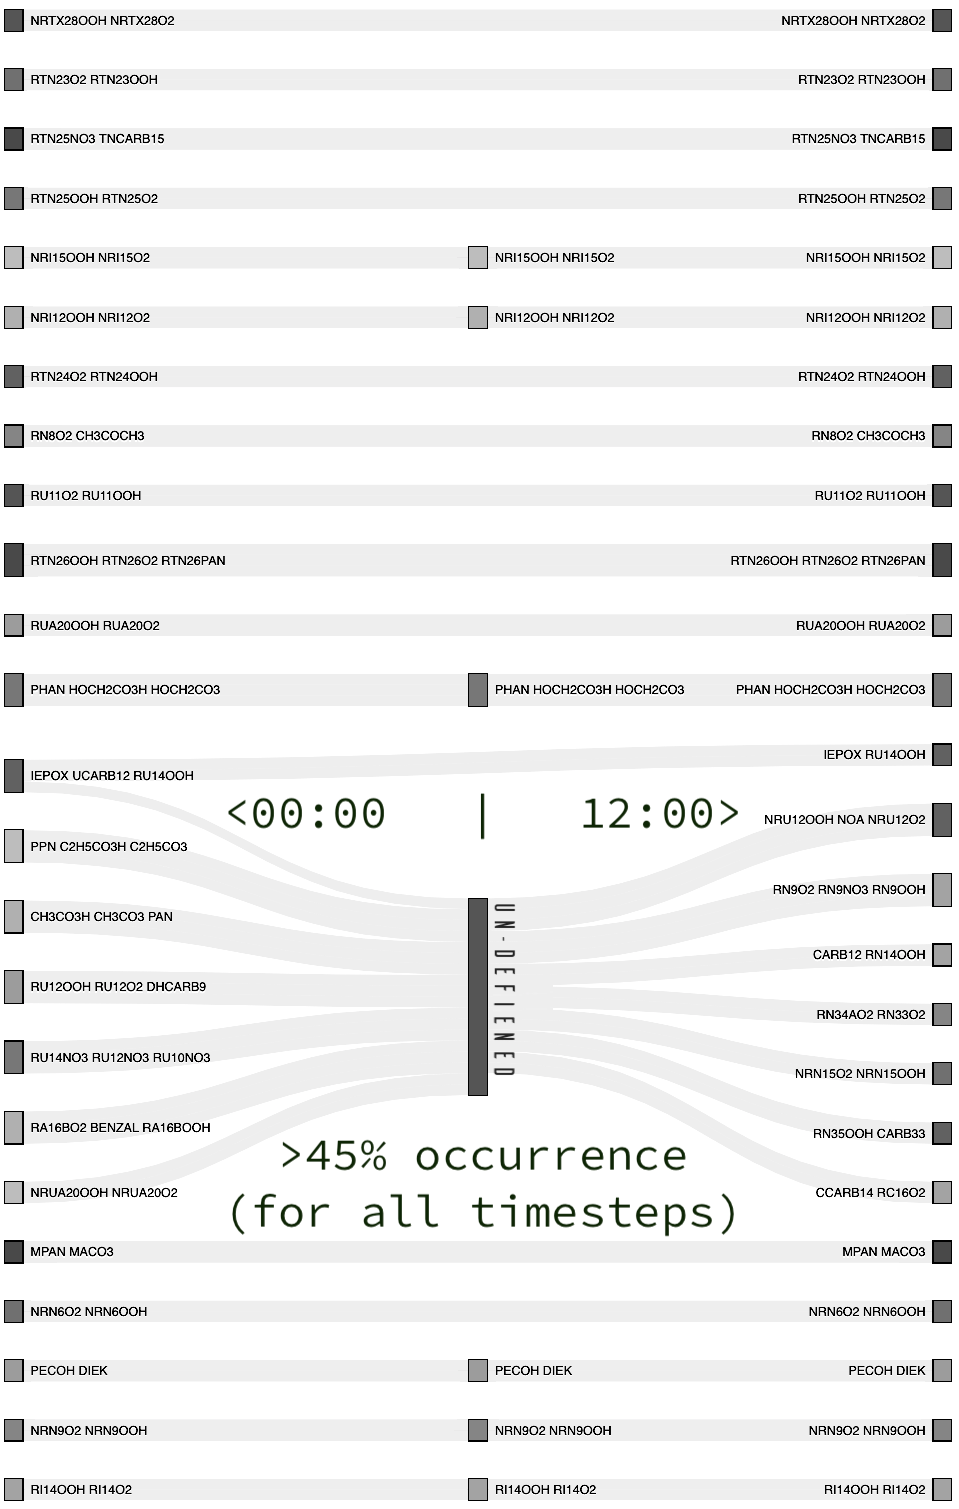
\includegraphics[width=.9\textwidth]{fig/alluvial.png}
\caption{\textbf{An alluvial diagram showing the changes in clusters between noon and midnight.} On the left are all groups that appear in >45\% of the midnight simulation results. On the right are groups which appear >45\% of the midday results. In the middle exist the clusters extracted which appear in >45\% of all runs. Here it is seen that there exist a series of species which may exist in the daytime or nighttime chemistry, but do not persist between both. Sizes represent the number of species and colours (greys) have no purpose other than to differentiate different items. }
\label{fig:alluvial}
\end{figure}



\subsection{Determining Cluster Suitabiltiy}
Having selected clusters that appear for most graphs in the network, it is now important to assess the suitability of each node for being lumped together. Using a normalised similarity matrix, we extract the values for each of the lumped groups, \autoref{tab:lumppair}. Here the best values are provided by the PECOH and DIEK species, \autoref{fig:lumppair}a. These both have linear decaying concentrations within the same order of magnitude. This is probably due to PECOH being the only precursor to DIEK, where DIEK accounts for 0.436\% of its total products. This makes them a suitable candidate for lumping.
\ce{HOCH2CO3H} and \ce{HOCH2CO3} make the worst possible lumping combinations. This is because the radical \ce{HOCH2CO3} can react with many of the inorganics, while \ce{HOCH2CO3H} can only dissociate into formaldehyde or react with OH to reproduce HOCH2CO3. Although these species both have differing profiles, of several orders of magnitude difference, their cyclic nature \ce{HOCH2CO3H <=>[OH][HO2] HOCH2CO3} most likely proved to trap the `flow' of the network, producing the cluster. Additionally there are also several clusters consisting of \ce{(N)RIxxOOH} and \ce{(N)RIxxO2} species. These are generally species formed from iso-alkanes (\autoref{appendix:correspondance}), and both produce acetaldehyde (\ce{CH3CHO}) as a product. Here the peroxy radical (\ce{R-O2}) produces a diurnal profile. Regardless of this, the cosine similarity is still relatively small. This may be attributed to the `flat' periods of slow decay that is experienced at nighttime (due to the reduction of available \ce{HO2} and \ce{NO}) which follow the loss trend of the peroxide (\ce{R-OOH}) species. Since OH addition and H-abstraction are both fast reactions these often form species with similar CRI numbers, the clustering algorithm often identifies peroxides and their peroxy radical equivalent as a group, \ce{RO2 <->[HO2][OH] ROOH}. \\


\begin{table}[H]
\centering
\begin{tabular}{l|cc}
\textbf{Sepecies Pair} & \textbf{Euclidean} & \textbf{Cosine}\\
\hline\hline
NRI15OOH NRI15O2 & 0.4624 & 0.2885 \\
\hline
NRI12OOH NRI12O2 & 0.4617 & 0.2986 \\
\hline
PHAN  HOCH2CO3 & 0.5103 & 0.9998 \\
HOCH2CO3H HOCH2CO3 & 0.8350 & 0.9892 \\
\hline
RI14OOH RI14O2 & 0.4922 & 0.2275 \\
\hline
NRN9O2 NRN9OOH & 0.4620 & 0.2818 \\
\hline
PECOH DIEK & 0.0172 & 0.0011 \\
\end{tabular}
\caption{A table of the \textbf{normalised} similarity values for the lumped species. Numbers closest to 1 show the worst possible paring in the mechanism, and numbers approaching 0 show the best. }
\label{tab:lumppair}
\end{table}


\begin{figure}[H]
\begin{subfigure}[t]{.5\textwidth}
  \centering
  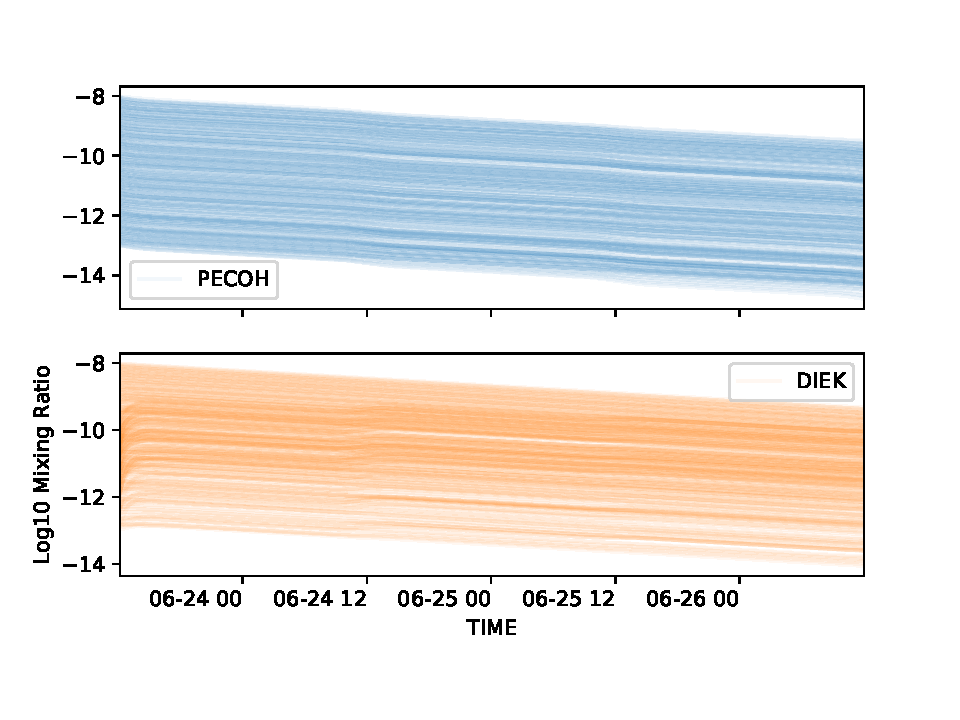
\includegraphics[width=\textwidth]{ensemble/PECOH-DIEK.pdf}
  \caption{\ce{  PECOH \ \ \ DIEK  }}
\end{subfigure}%
\begin{subfigure}[t]{.5\textwidth}
  \centering
  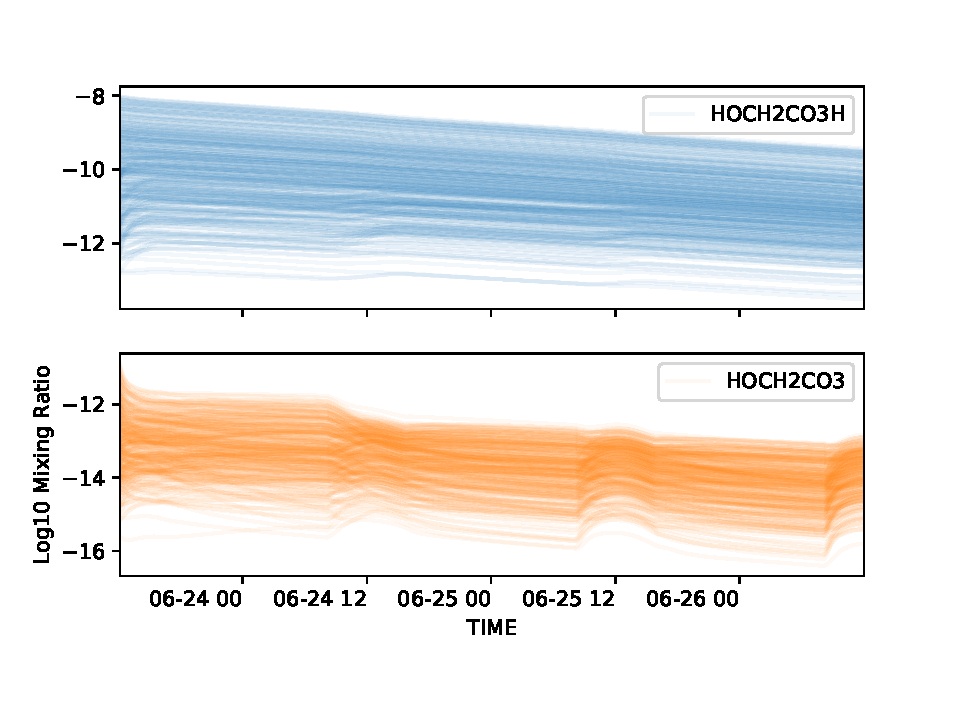
\includegraphics[width=\textwidth]{ensemble/HOCH2CO3H-HOCH2CO3.pdf}
  \caption{\ce{ HOCH2CO3H \ \ \ HOCH2CO3 }}
\end{subfigure}%\\

\begin{subfigure}[t]{.5\textwidth}
  \centering
  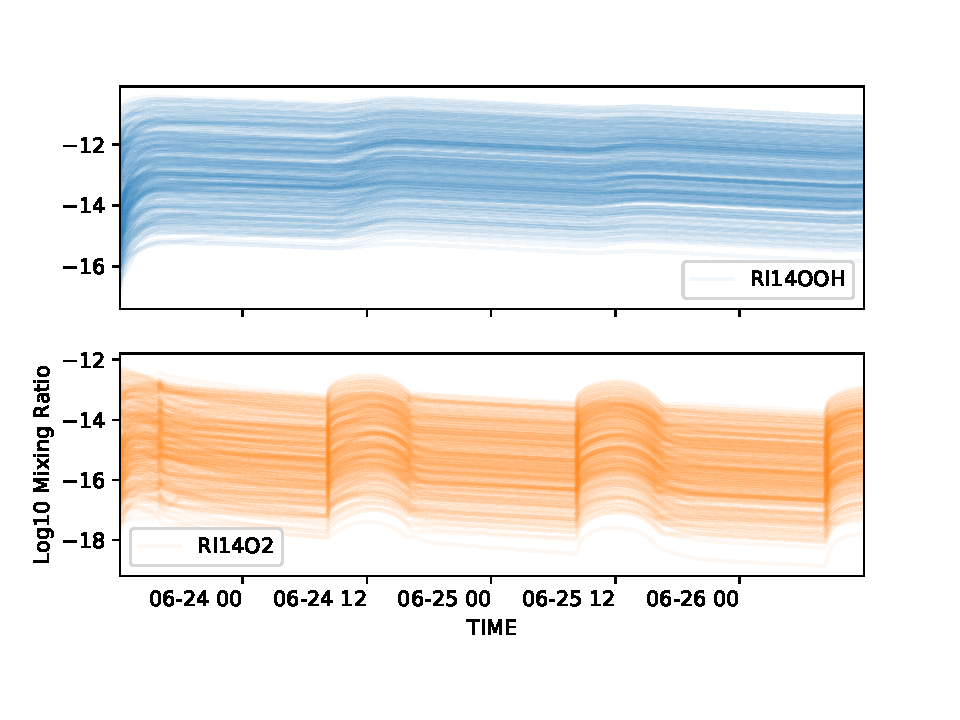
\includegraphics[width=\textwidth]{ensemble/RI14OOH-RI14O2.pdf}
  \caption{\ce{  RI14OOH \ \ \ RI14O2 }}
\end{subfigure}%
\begin{subfigure}[t]{.5\textwidth}
  \centering
  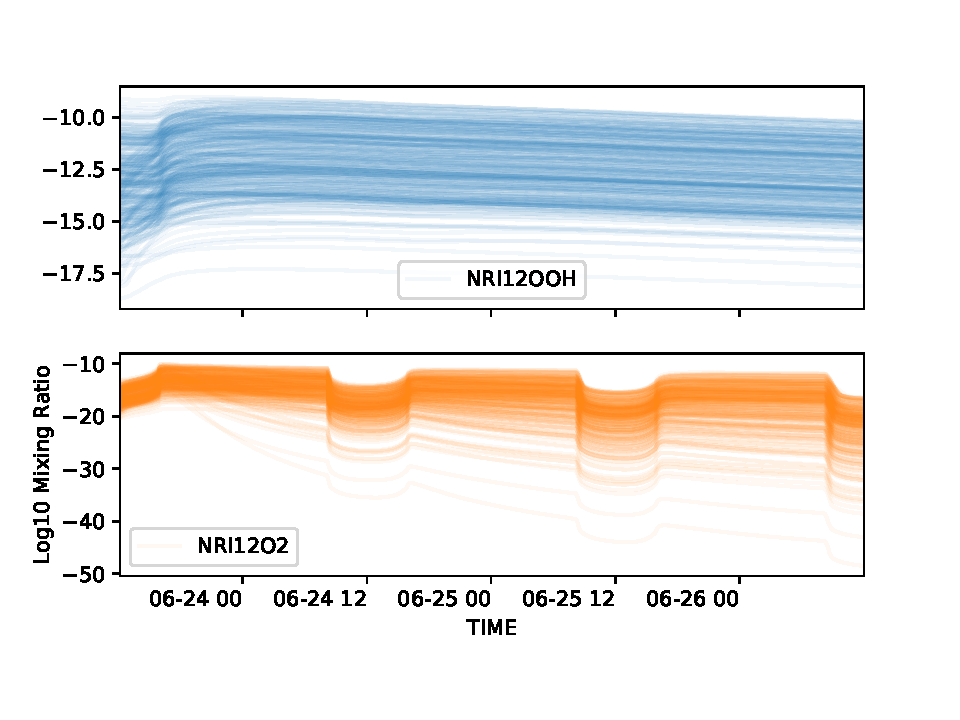
\includegraphics[width=\textwidth]{ensemble/NRI12OOH-NRI12O2.pdf}
  \caption{\ce{ NRI12OOH \ \ \  NRI12O2  }}
\end{subfigure}%\\
\caption{\textbf{Comparing the best and worst pairs from \autoref{tab:lumppair}}Time is in the format DD-MM HH}
\label{fig:lumppair}
\end{figure}





%
%
% df.index = pd.MultiIndex.from_tuples(...
%
% df.euclid = df.euclid/df.euclid.max()
% df.cosine = df.cosine/df.cosine.max()
%
%
%
% g = 'NRI15OOH NRI15O2,,NRI12OOH NRI12O2,,PHAN HOCH2CO3H,PHAN  HOCH2CO3,HOCH2CO3H HOCH2CO3,,RI14OOH RI14O2,,NRN9O2 NRN9OOH,,PECOH DIEK'.split(',')
%
%
% s =''
% for i in g:
%     try:
%         e = df.loc[tuple(sorted(i.split()))]
%         s+= '%s & %.4f & %.4f //\n'%(i,e.euclid,e.cosine)
%     except:
%         s+= ' & & //\n'
%
%
% print(s)
%
%
% g = 'NRI15OOH NRI15O2,NRI12OOH NRI12O2,PHAN HOCH2CO3H HOCH2CO3,RI14OOH RI14O2,NRN9O2 NRN9OOH,PECOH DIEK'.split(',')
%
%
% def get(x):
%     import zhdf
%     print (x)
%     return zhdf.new('lhs_general.h5',groupid = x,selection='spec',prodloss=False).spec.compute()
%
% import multiprocessing as mp
%
% gps = mp.Pool(50).map(get,range(0,300))
%
%
%
%
% g = 'RN27OOH RN37OOH,UDCARB20 UDCARB17,UDCARB14 UDCARB17,NRN9O2 NRN9OOH,PECOH DIEK'.split(',')
%
% g = 'C2H5CO3 CH3NO3,CH3CO3 CH3NO3,MACO3 CH3NO3'.split(',')
%
%
%
% g=['RTX24O2  RTX22O2']
%
%
% for i in g:
%     i = i.replace('-',' ').split()
%     print(i)
%
%     plt.clf()
%     ax = 0
%     del ax
%
%     for a in gps:
%         alpha = 0.06
%         d = np.log10(a[i])
%         try:
%             ax = d.plot(ax = ax,alpha = alpha,subplots=True,legend=False)
%         except:
%             ax=d.plot(alpha = alpha,subplots=True)
%
%     plt.ylabel('Log10 Mixing Ratio')
%     plt.savefig('-'.join(i)+'.pdf')





\newpage

\section{Conculsions}

\autoref{ch2} discussed graphs as a useful method for representing the chemistry within a mechanism. Building on that \autoref{ch3} showed that graph centrality metrics could be used to mathematically locate nodes (species) of importance from the chemical network from a chemical simulation. This chapter explores the chemical structure of the MCM network and uses graph clustering methods to locate groups of similar chemistry (\autoref{fig:imap2page}).

This process was trialled, using 300 randomly initiated simulations, on the CRI v2.2 mechanism \citep{cri}. In addition to graph clustering, we use cosine and Euclidean distances to compare the concentration magnitude and profile for species which may be lumped together. These are natural language processing techniques which allow the comparisons of two (temporal) arrays comparing their geometric distance and the angle between them.

For example, only six pairs of species were identified to be potentially lumped together. This has shown that in using the methodology presented, it is possible to located potential candidates -  although both the parameters and the sensitivity of grouping these within a chemical simulation need to be further explored. Future work should involve the use of real-world chemical scenarios, and clear optimisation criteria to which to benchmark the results against - if using CRI and the MCM this will likely be ozone-forming potential. Since CRI v2.0 has an additional five reduced states, it would be useful to attempt to reduce that and compare the results against the pre-existing mechanisms.

This chapter has shown a novel way for querying and representing a mechanism. This methodology needs to be further developed and applied to real-world chemistry before any conclusive comments on its applicability to atmospheric chemistry are made.
